% !TeX spellcheck = hu_HU
\documentclass[12pt,a4]{article}
\usepackage{xurl}
\usepackage{graphicx}
\usepackage{wrapfig}
\usepackage{lipsum}
\usepackage{amsmath}
\usepackage{amssymb}
\usepackage[super]{nth}
\usepackage{graphicx}
\usepackage[section]{placeins}
\usepackage{mdframed}
\usepackage{hyperref}
\usepackage{caption}
\usepackage{multirow}
\usepackage{subcaption}
\usepackage{indentfirst}
\usepackage{multicol}
\usepackage{mathtools}
\usepackage[figurename=Ábra]{caption}
\hypersetup{
	colorlinks=true,
	linkcolor=black,
	filecolor=magenta,      
	urlcolor=cyan,
	bookmarks=true,
	pdfpagemode=FullScreen,
}
\usepackage{array}
\newcolumntype{P}[1]{>{\centering\arraybackslash}p{#1}}
\newcolumntype{M}[1]{>{\centering\arraybackslash}m{#1}}

\hyphenation{op-er-and op-er-ands}

\def\magyarOptions{defaults=hu-min}
\PassOptionsToPackage{magyar}{babel}
\usepackage[inputenc=utf8]{uni8}

\begin{document}	
	
	\renewcommand*\contentsname{Tartalomjegyzék}	
	
	\begin{titlepage}
		\begin{figure}
			\centering
			\begin{minipage}{.5\textwidth}
				\centering
				
\includegraphics[width=.9\linewidth]{oelogo}
			\end{minipage}%
			\begin{minipage}{.5\textwidth}
				\centering
				
\includegraphics[width=.3\linewidth]{oe}
			\end{minipage}
		\end{figure}
		\vspace{0.5cm}			
		\begin{center}			
			\Large
			Óbudai Egyetem\\
			Neumann János Informatikai Kar\\
			
			\vspace*{0.5cm}
			
			\Huge
			\textbf{3D-s arckép rekonstrukciója egy 2D-s képből mesterséges intelligencia segítségével}
			\par\noindent\rule{\textwidth}{0.4pt}
			
			\vspace{0.5cm}
			\normalsize
			Reconstructing 3D face picture from single 2D picture supported by artificial intelligence
			
			\vspace{0.2cm}
			\large
			\today
			
			\vspace{1cm}
			
			Témavezető:\\
			\textbf{Vámossy Zoltán}\\
			Egyetemi docens
			
			\vspace{1cm}
			
			Készítette:\\
			\textbf{Gaál Bernát Ruben - HBGCXK\\
			Hua Nam Anh - DQ4LFK}					
		\end{center}
	\end{titlepage}
	\renewcommand*\contentsname{Tartalomjegyzék}
	\tableofcontents
	\newpage
	\par\noindent\rule{\textwidth}{0.4pt}
	\section*{Absztrakt}
     \emph{
		A közelmúltban a mélytanuláson alapuló 3D arcrekonstrukciós módszerek
		ígéretes eredményeket mutattak mind minőség, mind hatékonyság tekintetében. A neurális hálózatok tanítása azonban jellemzően nagy mennyiségű címkézett
		adatot igényel, ami magával vonzza a megfelelő erőforrásokat.
		A felsoroltak hiányában mi az alábbi megoldást javasoljuk. Egy gyengén
		felügyelt tanítású hálózatot, amit lehetséges kontrollálatlan környezetben készült képekkel betanítani.
		Ennek megvalósításához kettő már kész kutatás anyagát vettük igénybe. Az
		első, \cite{deca}DECA képes kezelni az arc kisebb részleteit, arckifejezéseit. A
		másik, a \cite{focus}FOCUS bemutatott egy korszerű megközelítést az arckép rekonstrukciójára kitakarások mellet. Ilyen kitakarások például a szemüveg és sapka. Ezek a kutatások nem csak korszerűek, de a NoW challenge teljesítményértekelései alapján bizonyítottan jól teljesítenek. Ezeket ötvözve egy robosztus, illetve realisztikus
		arcképek generálására alkalmas módszert mutatunk be ebben a tanulmányban.
		A rekonstrukció mellet implementáltunk egy arckép analízálására alkalmas módszert, amely képes eldönteni az arcképen lévő személy érzelmi
		állapotát és korát. Ezek köré egy felhasználó barát microservice alapú web
		applikációt biztosítunk, melynek szolgáltatásai felhőn üzelmelnek.
		}
	   \par\noindent\rule{\textwidth}{0.4pt}

    \section{Bevezetés}
        Az elmúlt évek során, egyre több figyelmet kaptak a digitális képfeldolgozáson alapuló technológiák az informatikában. 
        Mint ahogy \cite{survey}Araceli Morales és tsai. is megemlítették a munkájukban, hogy az arcfelismerő technológiák széles körben elterjedtek napjainkban, beleértve a biztonságot, animációt és egészségügyet. 
        Illetve, ezen szakmai területen mostanság felkapott, hogy 3D-s adatok implementálásával megkerüljék a 2D arckép által megszabott határokat, mivel a 2D-s kép képtelen az emberi arc geometriájának eltárolására.
        A 3D arcfelismerés sokkal pontosabb adatokat ad vissza, például pózban és megvilágításban, amelyek hátulütői a 2D-nek. Azonban ennek is vannak hátrányai, mint például, hogy sokkal nagyobb komplexitású képfeldolgozást igényel, ezáltal szűkítve a lehetőségeket.

        Az arcokat többféleképpen is lehet rögzíteni, például Stereo-vision rendszerekkel, amelyek két kamerát használnak. Ezek a kamerák ugyan arról az objektumról készítenek párhuzamosan képeket, majd ezeket összehasonlítva visszaadják a képen lévő egy pontnak a mélységét.

        Egy másik módszer a 3D lézerszkenner (pl. NextEngine, Cyberware), amelyet elsősorban ipari célokra fejlesztettek. Ipari termékek vizsgálatával szemben, az emberi arc feltérképezéséhez több feltételt kell figyelembe venni. Mivel az emberi arc nem lehet teljesen mozdulatlan, fontos, hogy a szkenner által készített felvétel időintervalluma csekély legyen.

        Röviden, a lézerszkenner fényhullámokat szór az objektumra, s ezek annak felszínéről visszaverődnek a szenzorra. A szenzor ezután kiszámítja az objektum felszínének távolságát az alapján, hogy mennyi idő alatt tette meg a teljes utat a hullám. Ezt a folyamatot $"Time\enspace of\enspace flight"$-nak szokás nevezni.

        A következő technológia a 3D-s adatok rögzítésére az RGB-D kamerák (pl. Kinect) használata. Ezek olyan RGB kamerák, amelyek rendelkeznek infravörös szenzorral, mely mélységi adatokat biztosít, ezáltal egy RGB képet ad vissza, amiben minden pixelhez tartozik egy mélységi érték.

        Bár, ezek a módszerek mind megfelelnek 3D-s adatok gyűjtésére, az első két megvalósítás hátránya, hogy előre megszabott feltételeknek megfelelő környezetet és drága felszereléseket igényel egy jó minőségű arc szkenneléshez. Ellenben, az RGB-D kamerák olcsóbbak és könnyebben használhatóak de a minőség korlátozott.

        A fent említett megközelítések általában költséges optimalizálási folyamatot igényelnek a jó minőségű 3D-s arc visszanyerése érdekében. Két évtized telt el \cite{blanzvetter}Blanz és Vetter úttörő munkája óta, amely először mutatta be hogyan lehet egyetlen képből rekonstruálni az arc 3D-s geometriáját. Azóta a 3D arcrekonstrukciós módszerek rohamosan fejlődtek, de a korábbi modellek csak az arc durva alakját tudták rekonstruktuálni és képtelenek voltak kinyerni az arckifejezéstől függő geometriai részleteket, mint például a ráncokat, amik fontosak a realisztikusság szempontjából.

        Később jöttek újabb modellek, melyek képesek voltak kiragadni a fent említett geometriai részleteket, azonban hátrányuk, hogy egy nagy volumenű, jó minőségű tanító adathalmazt követelnek. Illetve, egy másik hátrányuk, hogy inkonzisztens módon teljesítettek az kitakarásokkal szemben. A kitakarások mindenütt jelen vannak és eleve nehezen kezelhetőek az alakjuk, megjelenésük és a pozíciójuk sokfélesége miatt. Ezáltal okozott probléma az, hogy az arcmodell alkalmazkodik az eltakart arcrégióhoz, és ennek eredményeként a rekonstruált arc torz lesz. Ezért fontos nyitott kérdés marad annak eldöntése, hogy mely pixelek illeszkedjenek és melyek ne illeszkedjenek az arcra egy 3D arc rekonstrukciója során kitakarások jelenlétében. A közelmúltban számos olyan módszert javasoltak, amelyek gyengén felügyelt tanítású konvolúciós neurális hálózatokat(CNN) használnak a hatékony, robosztus és a fent említett kihívásokat leküzdő arcrekonstrukció eléréséhez.

        Tehát, a jelenlegi monokuláris 3D arcrekonstrukciós módszerek képesek finom geometriai részleteket visszaadni, azonban számos megkötéssel küzdenek. Egyes módszerek olyan arcokat generálnak, amelyeket nem lehet valósághűen animálni, mivel nem modellezik, hogy hogyan változnak a ráncok az arckifejezésekkel. Más módszerek kiváló minőségű szkennelt arcokat használnak tanításhoz, és nem jól általánosíthatóak a természetes körülményekben készült képekre. A Yao Feng és tsai. által bemutatott DECA model a legelső olyan megközelítés \cite{deca}, amely regresszálja a 3D arcformát és az animálható részleteket, amelyek egy személyre jellemzőek, de az arckifejezéssel változnak, ezáltal képesek az arc valósághű animálására.

        A kitakarásokkal szemben a legtöbb megközelítés a 3D arc illesztéséhez inverz renderelést alkalmaz egy adott eltakaró szegmentálásához. Ennek hátránya, hogy egy szegmentációs modellhez nagy mennyiségű címkézett adatra van szükség. Chunlu Li és tsai. \cite{focus} ezzel ellentétben egy olyan modellalapú megközelítést mutat be a 3D arc rekonstrukciójához, amely rendkívül robosztus az arcot kitakaró tényezőkkel szemben, de nem igényel semmilyen címkét a kitakarásokról a tanításhoz.

        Ebben a tanulmányban az a célunk, hogy egy olyan animálható 3D arcrekonstrukciós modellt készítsünk gyengén felügyelt tanulással, amely robosztus a kitakarások ellen, a fent említett DECA és FOCUS modellek segítségével. Ezt kiegészítve, bemutatunk egy arcképet elemző megoldást, mely visszaadja a célszemély érzelmi állapotát, illetve életkorát. Eszrevettük a munkánk elkészítése során, hogy a meglévő megoldásokat nehéz egy átlagos személynek kipróbálnia technikai tudás hiányában, így a fenti két szolgáltatás köré egy webapplikációt készítünk, amit felhőn üzelmeltetünk.\\

        Összefoglalva, ez a dokumentum az alábbi öt szempontot fogalmazza meg:
        \begin{itemize}
	       \item Bemutatunk egy CNN-alapú, egyetlen képen alapuló arcrekonstrukciós módszert, amely kihasználja a hibrid szintű képinformációt a gyengén felügyelt tanuláshoz.
	       \item Konzisztens műkődést biztosít különböző kitakarások mellet.
	       \item Az arckifejezésektől függő geometria adatok azonosításával egy animálható realisztikus 3D arcrekonstrukciót hozunk létre.
	       \item Arc elemzésére alkalmas megoldás.
	       \item Webapplikáció elkészítése és a szolgáltatások megfelelő mükődése a felhőn
        \end{itemize}

    \section{Előzetes kutatások}
	\subsection{Neurális hálózat}
    Ebben a fejezetben Abraham és tsai. munkája alapján bemutatjuk a neurális hálózatok működését.
    
	\label{NN}
	Az emberi agy bizonyítja a hatalmas neurális hálózatok létezését, amelyek sikeresen végeznek el kognitív, észlelési és irányítási feladatokat. Ilyen számításigényes feladat például az arcfelismerés, a beszéd és a testmozgás. Az agy hatékonyan kihasználja a masszív párhuzamosságot, számítási struktúrája nagymértékben párhuzamos és jó információfeldolgozási képességgel rendelkezik.
	
    \begin{figure}[h]	
		\centering
		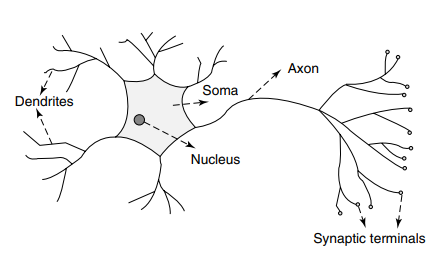
\includegraphics[width=1\linewidth]{neuron1}
        \label{fig:neuron1}
		\caption{Neuron felépítése. 
			Forrás:\cite{ann}}
	\end{figure}
 
	Az emberi agy több, mint 10 milliárd egymással összefüggő neuron gyűjteménye. Mindegyik neuron egy sejt \ref{fig:neuron1}, amely biokémiai reakciókat használ az információ fogadáshoz, feldolgozáshoz és továbbításhoz.
	
	Az idegrostok faszerű hálózatai, az úgynevezett dendritek kapcsolódnak a sejttesthez, ahol a sejtmag található. A sejttestből egyetlen hosszú rost nyúlik, melyet \textit{axon}nak neveznek. Az \textit{axon} szálakra és alszálakra ágazik, majd szinapszisain keresztül kapcsolódik más neuronokhoz. Az itt létrejövő szinaptikus kapcsolat erőssége határozza meg az emberi agy tanulását\cite{ann} .
	
	A jelek átvitele egyik neuronról a másikra a szinapszisoknál egy összetett kémiai folyamat, amelyben specifikus közvetítő anyagok szabadulnak fel a kapcsolódási pont küldői oldalán. A folyamat hatására a fogadó sejtben emelkedik vagy csökken az elektromos feszültség.
	
	\newpage
	\subsection{Mesterséges neurális hálózatok}
	A mesterséges neurális hálózatok (ANN-artificial neural networks) az előző fejezetben [\autoref{NN}] említett fejlettebb élő szervezetek agyát alkotó neuronokról kapták nevüket. 
	
	Mint azt \textit{Abraham} és tsai. \cite{ann} is említik, a neurális hálózatok alapvető feldolgozási elemeit mesterséges neuronoknak nevezzük, vagy csak egyszerűen neuronoknak vagy csomópontoknak. A neuron leegyszerűsített matematikai modelljében a szinapszisok hatásai kapcsolati súlyokkal vannak reprezentálva, amelyek szabályozzák a bemeneti jelek hatását.
	
	 A neuronok által mutatott nonlineáris karakterisztikát átviteli függvény segítségével ábrázoljuk. A neuron impulzusát ezután a bemeneti jelek súlyozott összegeként számíthatjuk ki az átviteli függvénnyel transzformálva.
	 
	  Egy mesterséges neuron tanulási képessége a súlyok megfelelő beállításával érhető el egy választott tanító algoritmus felhasználásával.
	\newline
	\newpage
	Egy tipikus mesterséges neuron és egy többrétegű neurális hálózat modellezése a \ref{fig:fig2}. ábrán látható. A \ref{fig:fig2}. ábrán szerint, ahogy a nyilak is mutatják, az $x_{1},...,x_{n}$ bemenetekről érkező jeláramlás egyirányúnak tekinthető csakúgy, mint a neuron kimeneti jelfolyama. A neuron kimeneti jelét \textit{O} a következő összefüggés adja:
	\begin{mdframed}
	\begin{align}
		&O = f(net) = f(\sum{j=1}^{n}w_{j}x_{j}) 
		\intertext{ahol $w_{j}$ a súly vektor és $f(net)$ az \textit{aktivációs} (átviteli) függvény. A \textit{net} változó a súly és a bementi vektorok skaláris szorzataként definiálható,}
		&net = w^{T}x = w_{1}x_{1} + ... + w_{n}x_{n}
		\intertext{ahol T egy mátrix transzponálását jelöli, és a legegyszerűbb esetben a kimeneti érték \textit{O} kiszámítható, mint}
		&O = f(net) = 
		\begin{cases}
			1,; ha ; w^{T}x ; \geq ; \theta \
			0, \text{különben} \
		\end{cases} \
	\end{align}
	ahol $\theta$-t \textit{küszöbszintnek} (threshold) nevezzük. Ezt a típusú aktivációs függvényt \textit{küszöb aktivációs függvénynek} nevezzük.
	
	\end{mdframed}
	
	
	\begin{figure}[h]%
		\centering
		\subfloat[\centering Mesterséges neuron]{{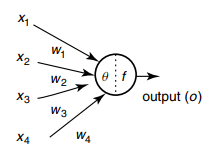
\includegraphics[width=5cm]{artificialNeuron} }}%
		\qquad
		\subfloat[\centering Többrétegű neurális háló]{{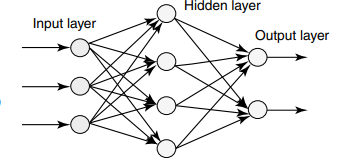
\includegraphics[width=5cm]{multilayered} }}%
		\caption{Mesterséges neuron felépítése és egy többrétegű neurális háló \newline\centering Forrás: \cite{ann}}%
		\label{fig:fig2}%
	\end{figure}
	\newpage
	A \textit{küszöbfüggvényhez} hasonlóan más aktivációs függvényekkel is előállítható az adott neuron bemenetre kapott válasz. Ilyen függvények a 
	\begin{itemize}
		\item lineáris,
		\item szigmoid,
		\item tangens hiperbolikusz.
	\end{itemize}

	\begin{figure}[h]	
		\centering
		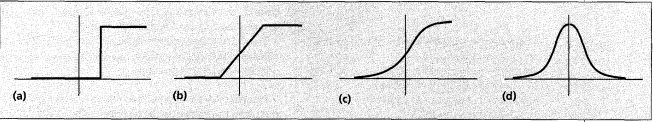
\includegraphics[width=1\linewidth]{fuggvenyek}
		\caption{(a) küszöbfüggvény, (b) lineáris, (c) szigmoid, (d) Gauss 
			\newline\centering Forrás:\cite{ann2}}
		\label{fuggvenyek}
	\end{figure}
	
	\begin{mdframed}
	Ma az egyik leggyakrabban használt aktivációs függvény a szigmoid \cite{ann4}, melyet a következő képlettel határoznak meg:
	\begin{align}
		&y = \frac{1}{1 + e^{-(a - \theta)b}}
	\end{align}
	ahol \textit{a} az aktiválás, \textit{b} pedig a görbe alakját szabályozza.
	\end{mdframed}
	
	\subsection{Neurális hálózat architektúra}
	
	Bár a mesterséges neuron működési elvei és 
	egyszerű szabályrendszere elsőre talán nem tűnik érdekesnek, azonban e modellek teljes potenciálja és számítási teljesítménye akkor kel életre, 
	amikor mesterséges neurális hálózatokká
	kezdjük őket összekapcsolni \ref{fig:fig2}. ábrán. 
	Ezek a mesterséges neurális hálózatok 
	kihasználják az egyszerű tényt, 
	hogy a komplexitás néhány alapvető
	szabályból tud növekedni.
	
	A mesterséges neurális hálózatok 
	képesek komplex, valós problémák megoldására azáltal
	, hogy 
	alapvető építőelemeikben (\textit{mesterséges neuronok}) feldolgozzák az információt nemlineáris,
	elosztott, párhuzamos és lokális módon.
	
	Krenker és tsai. 
	\cite{krenker} munkája alapján az egyes mesterséges 
	neuronok összekapcsolásának módját 
	\textit{topológiának}, \textit{architektúrának} 
	vagy \textit{gráfnak} nevezzük. A tény, 
	hogy az összekapcsolás
	számos lehetséges módon történhet több alkalmazható topológiát eredményez, amelyek két fő csoportra bonthatók. 
	
	A \ref{fig:topologies}. ábra ezt a két topológiát mutatja. Az ábra bal oldala egy egyszerű feedforward topológiát ábrázol, ahol az információ a bemenetekről kimenetekre áramlik egyirányúan. Az ábra jobb oldala pedig egy egyszerű rekurzív (\textit{recurrent}) topológiát ábrázol, ahol az információ egy része nem csak egy irányban áramlik a bemenetről a kimenetre, hanem ellenkező irányban is.

	Fontos megemlíteni, hogy a mesterséges neurális hálózat könnyebb kezelése és matematikai leírása érdekében az egyes neuronokat rétegekbe soroljuk. A \ref{fig:topologies}. ábrán láthatjuk a bemeneti, a rejtett és a kimeneti réteget.
	\begin{figure}[h]	
		\centering
		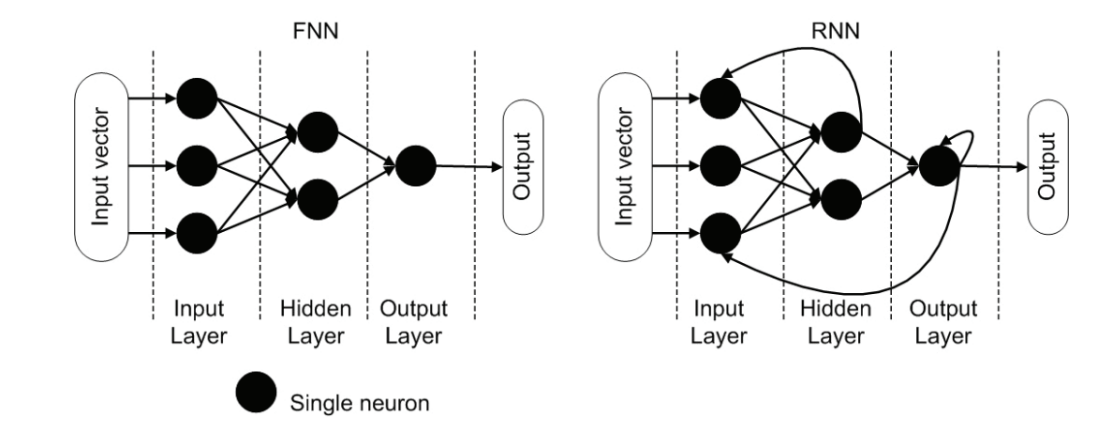
\includegraphics[width=1\linewidth]{topologies}
        \label{fig:topologies}
		\caption{Feed-forward (FNN) és recurrent (RNN) \newline\centering  neurális hálózati topológiák. 
			Forrás:\cite{krenker}}
	\end{figure}

	A háló input rétegében minden neuron kapcsolatban áll a \textit{rejtett} (köztes) réteggel, így tovább adhatja a bemenetként kapott adatokat. A bemeneti réteg neuronjai súlyozott szinapszisokkal kapcsolódnak a belső rétegekhez.\\
	
	A mesterséges neurális hálózat 
	topológiájának kiválasztásával és 
	felépítésével még csak a feladataink 
	felét fejeztük be mielőtt a hálót az 
	adott probléma megoldására használhatnánk.
	Csakúgy, mint a biológiai neurális hálózatoknak
	is meg kell tanulniuk a megfelelő válaszokat különböző környezeti bemenetekre, a mesterséges neurális hálózatoknak is pontosan ezt kell tenniük.
	
	
	A következő lépés tehát, hogy \textit{betanítsuk} a mesterséges neurális hálózatot a helyes válaszokra.
	Erre négy lehetőségünk van:
	\begin{itemize}
		\item a felügyelt
		\item a felügyelet nélküli
		\item a megerősítéses
		\item és a hibrid
	\end{itemize}
	tanulás.
	
	 Függetlenül attól, hogy melyik módszert választjuk, a tanulás feladata, hogy a tanulási adatok alapján beállítsuk a súlyok és az előfeszítések értékeit, hogy minimalizáljuk a 
	költségfüggvényt.
	
	\subsection{Neurális hálók tanítása}
    Ebben a fejezetben \cite{krenker} és tsai. munkája alapján mutatjuk be a nerális hálózatok tanítási módszereit.
 
	A tanulási folyamat \cite{ann2} az ANN kontextusában a
	hálózat architektúrája és a kapcsolati súlyok frissítéseként értelmezhető annak érdekében, hogy a háló hatékonyan tudjon elvégezni egy adott feladatot.
	A hálózatnak a rendelkezésre álló tanító mintákból kell megtanulnia a kapcsolati súlyokat. A teljesítmény idővel javul a súlyok iteratív frissítésével.
	Az ANN-eket automatikus, példákból való tanulása teszi 
	vonzóvá és érdekessé. Szakértők által definiált szabályok helyett az ANN-ek a mögöttes szabályokat tanulják meg (pl. bemeneti-kimeneti kapcsolatokat) a megadott reprezentatív példák gyűjteményéből.
	
	\subsubsection{Felügyelt tanulás (\textit{supervised learning})}
	
	A felügyelt tanulás egy olyan gépi tanulási (\textit{machine learning}) technika, amely egy mesterséges neurális hálózat paramétereit tanítási
	adatokból állítja be. A tanuló ANN feladata, hogy beállítsa paramétereinek értékét bármely érvényes bemeneti értékre, miután látta a kimeneti értéket.
	A képzési adatok a bementi és a kívánt kimeneti értékek párjaiból állnak, amelyeket adatvektorokban ábrázolnak.
	
	
	A felügyelt tanulást \textit{klasszifikációnak} is nevezhetjük, ahol \textit{osztályozók} széles skálája áll rendelkezésünkre, amelyek mindegyikének megvannak az erősségei és gyengeségei.
	A felügyelt tanulás egy
	adott problémájának megoldásához különböző lépéseket kell figyelembe venni.
	
	 Az első lépésben meg kell határoznunk a tanítási minták típusát. A második
	lépésben olyan tanítási adathalmazt kell gyűjtenünk, amely kielégítően leírja az adott problémát.
	A harmadik lépésben az összegyűjtött tanítási adathalmazt
	olyan formában kell leírnunk, amely érthető a kiválasztott ANN számára. A negyedik lépésben elvégezzük
	a tanítást. Ezután tesztelhetjük a tanult ANN teljesítményét a teszt (validációs) adathalmazzal.
	A validációs adathalmaz olyan adatokból áll, amelyeket a tanulás során nem vezettünk be a mesterséges neurális hálózatba.
	
	\subsubsection{Felügyelet nélküli tanulás (\textit{unsupervised learning})}
	
	A felügyelet nélküli tanulás egy olyan gépi tanulási (\textit{machine learning}) technika, amely egy ANN paramétereit megadott adatok és egy minimalizálandó 
	költségfüggvény alapján állítja be. A költségfüggvény bármilyen függvény lehet, amit a feladat határoz meg.
	
	
	Felügyelet nélküli tanulást leginkább olyan alkalmazásokban használnak, amelyek a becslési problémák körébe tartoznak, mint például a statisztikai modellezés, filterezés és a klaszterezés. A felügyelet 
	nélküli tanulás során arra törekszünk, hogy meghatározzuk, hogyan szerveződnek az adatok. Ez a felügyelt és a megerősítéses tanulástól abban különbözik, hogy az ANN csak \textit{címkézetlen} mintákat kap. A felügyelet nélküli tanulás egyik gyakori formája a klaszterezés, ahol az adatokat hasonlóságuk alapján próbáljuk különböző klaszterekbe sorolni.
	
	\subsubsection{Megerősítéses tanulás (\textit{reinforcement learning})}
	
	A megerősítéses tanulás egy olyan gépi tanulási (\textit{machine learning}) technika, amely egy olyan
	mesterséges neurális hálózat paramétereit állítja be, ahol általában az adatok nincsenek előre megadva, hanem a környezettel való kölcsönhatásokból generálódnak. A megerősítéses tanulás azzal foglalkozik, hogy egy mesterséges neurális hálózatnak hogyan kellene viselkednie egy adott környezetben annak érdekében, hogy maximalizálja a hosszú távú 
	eredményeket.
	
	Miután a maximalizálandó visszatérési függvényt meghatároztuk, a megerősítéses tanulás számos algoritmust használ a maximális visszatérést eredményező szabályok meghatározására. Az első lépésben egy naiv \textit{brute force} algoritmus kiszámítja a \textit{visszatérési függvény}t minden lehetséges szabályhoz és kiválasztja azt, amelyik a legnagyobb visszatéréssel rendelkezik. Ennek az algoritmusnak nyilvánvaló gyengesége a rendkívül magas vagy akár végtelen számú lehetséges szabály esetében rejlik. Ez a gyengeség kiküszöbölhető érték függvényes megközelítésekkel vagy közvetlen szabály becslésekkel. Az értékfüggvényes megközelítések megpróbálnak
	egy olyan szabályrendszert találni, amely maximalizálja a visszatérést.
	
	Ezek a módszerek konvergálnak a helyes becslésekhez egy rögzített szabály esetén, és az optimális szabály megtalálására is használhatóak. Az értékfüggvényes megközelítéshez hasonlóan a közvetlen szabály becslés is képes megtalálni az optimális szabályt.

    \subsubsection{Átviteli tanítás}
    
     A hagyományos gépi tanulási módszerek egyik feltételezése, hogy a tanítási és tesztelési adatok ugyanabból a tartományból származnak, így a bemeneti jellemzőtér és az adatok eloszlási jellemzői megegyeznek. Néhány valós gépi tanulási forgatókönyvben azonban ez a feltételezés nem áll fenn. Vannak olyan esetek, amikor a képzési adatok gyűjtése drága vagy nehézkes. Ezért nagy teljesítményű tanulók létrehozására van szükség, amelyeket különböző tartományokból könnyebben beszerezhető adatokkal tanítanak. Ezt a módszert átviteli tanulásnak nevezzük \cite{tl}.

     Az átviteli tanítás alapvető célja a modell fejlesztésének felgyorsítása egy meglévő modellből kiindulva és annak tovább hangolása a specifikus problémára.
 
	\subsection{Konvolúciós neurális hálózatok}
	\begin{figure}[h]	
		\centering
		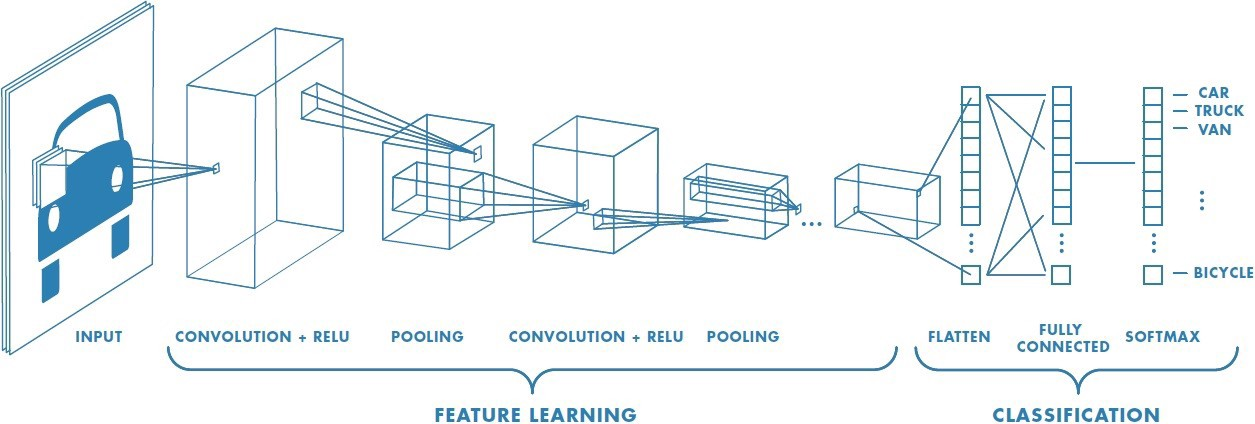
\includegraphics[width=1\linewidth]{CNN}
        \label{fig:cnn}
		\caption{CNN(Convolutinal Neural Network)}
	\end{figure}
	Indolia és tsai. \cite{CNN} értelmezésében a konvolúciós neurális hálózat (CNN) egy
	mélytanulási megközelítés, amelyet széles körben használnak komplex problémák megoldására és felülmúlja a hagyományos gépi
	tanulási megközelítéseket.
	
	A konvolúciós neurális hálózat mély feed-forward architektúrával rendelkezik, és jobban képes általánosítani, mint a teljesen összekapcsolt rétegekkel rendelkező hálózatok.
	
	A CNN, mint a hierarchikus jellemző detektorok biológiailag inspirált koncepciója, képes nagymértékben megtanulni
	absztrakt jellemzőket és hatékonyan képes azonosítani az objektumokat.
	
	A CNN-t az alábbi előnyökkel rendelkezik más klasszikus modellekkel szemben:
	
	  A CNN-ek alkalmazásának legfőbb előnye a súlymegosztás koncepciójában rejlik
	, amelynek köszönhetően a betanítandó paraméterek száma jelentősen csökken, ami jobb általánosításhoz vezet. 
	A kevesebb paraméter miatt a CNN egyszerűen betanítható, és nem szenved túlillesztéstől(overfitting).
	
	
	Másodszor, az osztályozási szakasz beépül a jellemző kinyerési szakaszba. Mindkét szakasz használ tanulási folyamatot.
	
	
	Harmadszor, a mesterséges neurális hálózat általános modelljeinek felhasználásával nagy hálózatokat sokkal nehezebb megvalósítani,
	mint CNN-ben.
	
	
	A CNN-eket széles körben használják különböző területeken figyelemreméltó
	teljesítményüknek köszönhetően, mint például a képosztályozás, a tárgyak felismerése, az arcfelismerés, a beszéd
	felismerés, járműfelismerés stb.
	
	\subsubsection{A konvolúciós neurális hálózat általános modellje}
    Ebben a fejezetben Indolia és tsai. \cite{CNN} munkéja alapján bemutatjuk a CNN-ek általános modelljét.
 
	\subsubsection{Általános modell}
	Az ANN általános modellje egyetlen bemeneti és kimeneti réteggel,
	valamint több rejtett réteggel rendelkezik.
	
	Egy bizonyos 
	neuron fogadja az X bemeneti vektort, és Y kimenetet állít elő azáltal,
	hogy valamilyen F függvényt hajt végre rajta az alábbi általános egyenlet alapján (\ref{eq1}).
	\begin{mdframed}
	\begin{equation}
    \label{eq1}
			F(X, W) = Y
	\end{equation}
	,ahol W a súlyvektor, amely a két neuron közötti összeköttetés erősségét jelöli két szomszédos réteg között.
 	\end{mdframed}

	A kapott súlyvektor most már felhasználható a képosztályozáshoz.
	
	Jelentős mennyiségű irodalom létezik a képek pixelalapú osztályozásával
	kapcsolatban, azonban az olyan kontextuális információk, mint a kép alakja vagy 
	a kép formája jobb eredményt adnak.
	
	A CNN a kontextuális információkon alapuló osztályozási képessége miatt kap egyre nagyobb figyelmet.\\
	
	
	A CNN általános modellje négy komponensből áll, nevezetesen 
	\begin{itemize}
		\item konvolúciós réteg
		\item pooling réteg
		\item aktivációs függvény
		\item teljesen összekapcsolt réteg
	\end{itemize}
	Az egyes komponensek működését az alábbi [\ref{fig:cnnelem}.] ábra szemlélteti.
	
	\begin{figure}[h]	
		\centering
		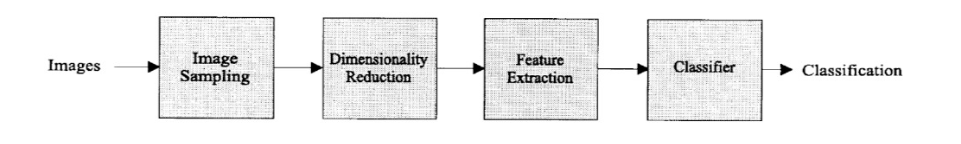
\includegraphics[width=1\linewidth]{element}
        \label{fig:cnnelem}
		\caption{\cite{CNN} A CNN elemi összetevői}
	\end{figure}

	
	\subsubsection{Konvolúciós réteg}
	
	Az osztályozandó képet a bemeneti rétegnek adjuk meg, a kimenet pedig az előre megjósolt osztálycímke, amelyet a képből kinyert jellemzők alapján számítunk ki.
	
	
	A következő rétegben lévő egyes neuronok az azt követő rétegben lévő neuronokhoz kapcsolódnak. Ezt a helyi korrelációt receptív mezőnek nevezzük.
	
	
	A bemeneti kép lokális jellemzőit a receptív mező segítségével nyerjük ki. Az előző rétegben egy adott régióhoz tartozó neuron receptív mezeje egy súlyvektort alkot, amely a sík minden pontján egyenlő marad, ahol a sík a következő rétegben lévő neuronokra utal. Mivel a síkban lévő neuronok azonos súlyokkal rendelkeznek, így a különböző helyeken előforduló hasonló jellemzők a bemeneti adatokon belül felismerhetők.
	
	\begin{figure}[h]	
		\centering
		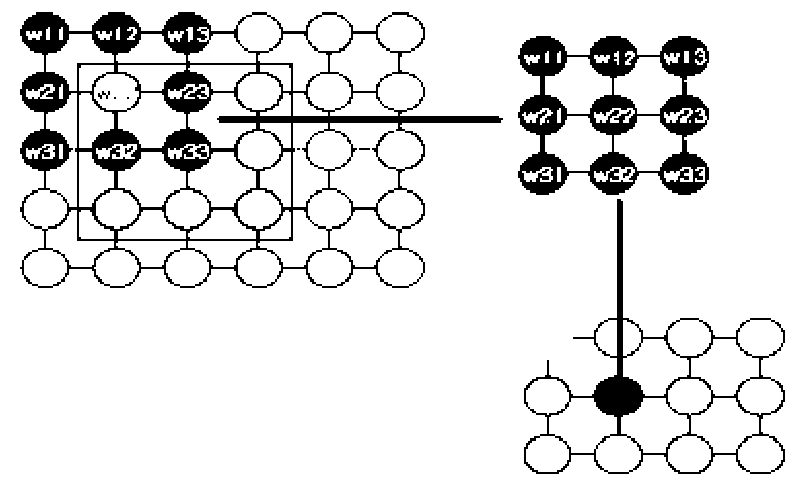
\includegraphics[width=0.7\linewidth]{receptiv}
		\caption{\cite{CNN} Az adott neuron receptív mezeje a következő rétegben}
	\end{figure}
		\newpage
	A súlyvektor, más néven szűrő vagy kernel a bemeneti vektoron csúszik át a \textit{featuremap} létrehozásához.
	A szűrő vízszintes és függőleges irányú csúsztatásának módszerét nevezzük konvolúciós műveletnek. A helyi receptív mező jelensége miatt a betanítható paraméterek száma jelentősen csökken.
	
	A következő rétegben az (i,j) helyhez tartozó $A_{ij}$ kimenet konvolúciós
	művelet alkalmazása után kerül kiszámításra az alábbi képlet segítségével:
	\begin{mdframed}
	\begin{align}
		a_{ij} = \sigma((W * X)_{ij} + b)
	\end{align}
	, ahol X a rétegnek adott bemenet, W a bemeneten áthaladó szűrő vagy kernel,
	b az eltolás, * a 
	a konvolúciós műveletet, és $\sigma$ a hálózatba bevezetett non-linearitást jelöli.
	\end{mdframed}
	
	\subsubsection{Összevonó réteg}

	A konvolúciós réteget összevonó (pooling) vagy 
	almintavételező (sub-sampling) \cite{CNN} réteg követi.
	A \textit{pooling} technika használatának fő előnye, hogy 
	jelentősen csökkenti a betanítható paraméterek számát,
	és bevezeti a fordítási invarianciát. 
	
	
	Az összevonás (\textit{pooling}) művelet elvégzéséhez kiválasztunk egy ablakot,
	és az abban az ablakban lévő bemeneti elemeket átadjuk
	egy összevonó (\textit{pooling}) függvénynek. a [8. ábrán] látható módon.
	
	\begin{figure}[h]	
		\centering
		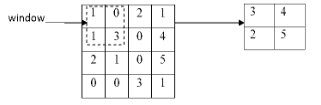
\includegraphics[width=0.7\linewidth]{pooling}
		\caption{\cite{CNN} 2 x 2 ablak kiválasztásával végzett összevonási művelet}
	\end{figure}
	
	\newpage
	
	A pooling függvény egy másik kimeneti vektort generál.
	
	
	Létezik néhány összevonási technika, mint például az átlagos összevonás (\textit{average pooling}). 
	és a \textit{max-pooling}, amelyek közül a \textit{max-pooling} a leggyakrabban használt módszer,
	mely jelentősen csökkenti a leképezés méretét.
	
	
	A hibák kiszámítása során a hiba nem terjed vissza a győztes egységre.
	
	\subsubsection{Teljesen összekapcsolt réteg}
	
	A teljesen összekapcsolt réteg \cite{CNN} hasonló a hagyományos modellek teljesen összekapcsolt hálózatához.
	
	
	Az első
	fázis kimenete (a konvolúciót és a összevonást ismétlődően tartalmazza) a teljesen összekapcsolt rétegbe kerül, és a súlyvektor és bemeneti vektor pontproduktumát számoljuk ki a végeredmény kiszámítása érdekében.
	
	
	A \textit{gradiens süllyedés}, más néven kötegelt módú tanulás vagy offline algoritmus, csökkenti a költségfüggvényt a költség becslésével egy teljes tanítói adathalmaz felett, és a paramétereket csak egy korszak után frissíti, ahol egy korszak a teljes adathalmaz átfutásának felel meg.
	Ez globális minimumokat eredményez, de ha a képzési adathalmaz mérete nagy, akkor a hálózat tanításához szükséges idő
	jelentősen megnő. A költségfüggvény
	\\
	csökkentésének ezt a megközelítését felváltotta a \textit{sztochasztikus gradiens süllyedés}.
	\subsubsection{Aktivációs függvény}
	
	
	Számos szakirodalom létezik, amely a hagyományos gépi tanulási algoritmusokban
	szigmoid aktivációs függvényt használ.
	A nemlinearitás bevezetése érdekében a Rectified Linear Unit (ReLU) \cite{CNN} használata jobbnak bizonyult az előbbinél
	két fő tényező miatt. 
	
	Először is, a ReLU parciális deriváltjának kiszámítása egyszerű. 
	Másodszor, miközben figyelembe vesszük
	a képzési időt mint az egyik tényezőt, a telítődő nemlinearitások, mint a szigmoid lassabbak, mint a nem telítődő nemlinearitások, mint a ReLU.
	 Harmadszor, ReLU nem engedi, hogy a gradiensek eltűnjenek, de a ReLU hatékonysága romlik, ha nagy gradiens áramlik át a hálózaton, és a súly frissítése miatt a neuron nem aktiválódik, ami a \textit{Dying ReLU} problémához vezet, amely egy jelentős probléma. 
	 
	 Ez a probléma megoldható a \textit{Leaky ReLU} segítségével, ha $x>0$, a függvény aktiválódik.
	mint $f(x)= x$, ha pedig $x<0$, akkor a függvény $\alpha x$-ként aktiválódik, ahol $\alpha$ egy kis konstans.

    \subsection{Reziduális Neurális Hálózatok}
    
    \begin{figure}[h]	
 		\centering
 		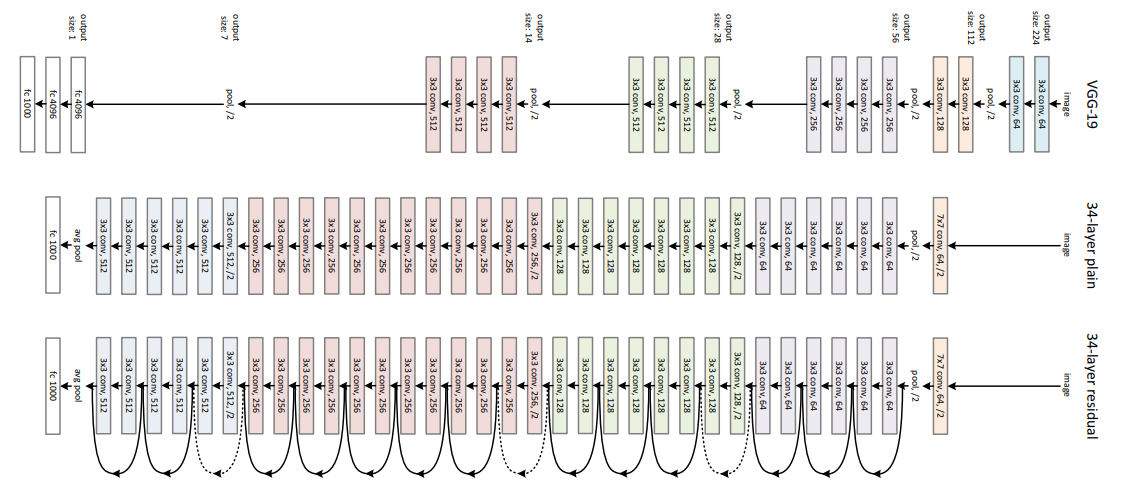
\includegraphics[width=1\linewidth]{ResNet}
 		\caption{ResNet architektúrák felépítése. (felülről a 3.)
 			Forrás:\cite{resnet}}
        \label{fig:resnet}
 	\end{figure}
    
    A mélyebb neurális hálózatok nehezebben taníthatóak. Mivel amikor növeljük a rétegek számát, a mélytanulásban egy gyakori probléma merül fel, amit eltűnő/robbanó gradiensnek neveznek. Ennek hatására a gradiens 0 vagy túl nagy lesz. Így amikor növeljük a rétegek számát, a hibaarány is nő. 
    
    Ennek a problémának a megoldására He et al. \cite{resnet} bemutattak egy reziduális (maradékos) tanulási keretrendszert, amely megkönnyíti azon hálózatok tanítását, amelyek lényegesen mélyebbek a korábban használtakhoz képest. 

     A rétegeket kifejezetten úgy alakították át, hogy a rétegek a réteg bemeneteire hivatkozva maradványfüggvényeket tanulnak a nem hivatkozott függvények helyett. Ezek a reziduális hálózatok könnyebben optimalizálhatók, és pontosságot nyerhetnek az jelentősen megnövelt mélységből fakadóan.

    \newpage
    \subsubsection{Reziduális blokkok}
    
    
    \begin{figure}[h]	
 		\centering
 		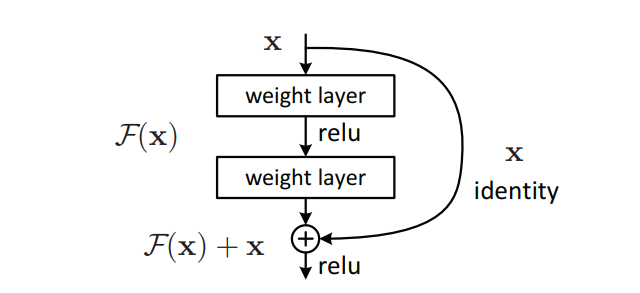
\includegraphics[width=1\linewidth]{Residual-Block}
 		\caption{He et al. által javasolt reziduális blokk felépítése.
 			Forrás:\cite{resnet}}
        \label{fig:resblock}
 	\end{figure}
  
    Az eltűnő/explodálódó gradiens problémájának megoldására bevezették a Reziduális/Maradék blokkokat. A hálózatban úgynevezett kihagyásos kapcsolatok jönnek létre. A kihagyásos kapcsolat egy réteg aktivációit úgy kapcsolja össze a további rétegekkel, hogy közben néhány réteget kihagy. Ez egy reziduális blokkot képez. A reziduális hálózatok ezen reziduális blokkok egymásra halmozásával jönnek létre. Az ilyen típusú kihagyásos kapcsolatok hozzáadásának előnye, hogy ha bármelyik réteg károsítja az architektúra teljesítményét, akkor azt a regularizáció kihagyja. Ez tehát egy nagyon mély neurális hálózat tanítását eredményezi az eltűnő/robbanó gradiens okozta problémák nélkül. 


    A saját megvalósításunkban egy előtanított 50 rétegű reziduális hálózatot átviteli tanítással tanítottunk tovább és finomhangoltuk azt a bemenetként átatott kép személyspecifikus jellemzőinek kinyerése érdekében.
    
    \section{Deep Learning módszerek}
	
	Az előző szakaszok [\nameref{3d}] 2D-ből 3D arc rekonstrukciós módszerei \textit{modelleket} használnak az előzetes tudás megtestesítésére \cite{survey}: a statisztikai modellillesztési módszerek tartalmaznak egy geometriai (és általában textúra) modellt, a fotometriai módszerek pedig a
	az arc fényvisszaverő képességét. 
	
	
	Ezzel szemben a mély tanulási módszerek
	közvetlenül tanulják meg a 2D kép és a 3D arc közötti leképezést, az előzetes ismeretek felhasználásával a betanított hálózatokban.
	
	
	Több indokból is előnyösebb mély tanulási módszerekkel dolgozni.\cite{3dmm}A modellezési oldalon a nemlineáris, mély reprezentációk használata lehetőséget nyújt arra, hogy felülmúljuk a klasszikus lineáris vagy multi-lineáris modelleket az általánosítás szempontjából, tömörség és specifikusság tekintetében \cite{styner}.
	
	
	A paraméter becslési oldalon ki tudjuk használni a mély hálózatok előnyeit, a gyorsaságot és a robusztusságot, hogy megbízható teljesítményt érjünk el a nem ellenőrzött képeken.
	
	\begin{figure}[h]	
		\centering
		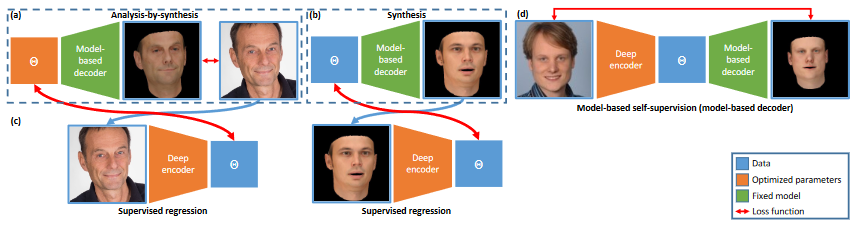
\includegraphics[width=1\linewidth]{deep}
		\caption{A klasszikus analízis-szintézis és a mélytanulási megközelítések közötti kapcsolat. 
			Forrás:\cite{3dmm}}
	\end{figure}
	
	\newpage
	\subsection{Deep Face modellek}
    Ebben az alfejezetben a deep face modellezési módszereket mutatjuk be \cite{3dmm} Egger és tsai. munkája alapján. \\
 
	A hagyományos modellezési technikák célja, hogy
	az arc alakját, arckifejezését és megjelenését $w$ vektorként reprezentálják egy
	alacsony dimenziós látens térben $\mathbb{R}^d$ . A vetítés (illetve rekonstrukció) ebből a latens térből lineáris vagy multi lineáris műveletekkel definiálható, és úgy is felfogható, mint a nagy-dimenziós információ kódolása (ill.
	dekódolása) a $\mathbb{R}^d$ térben.
	
	
	A mélytanulás új eszközt nyújt a 3DMM-ek építéséhez, amely nemlinearitást használ mind a kódolóban és a dekódolóban. Az ilyen \textit{morphable} modellek létrehozása egy jelenleg nagyon aktív kutatási terület.
	Az alak és textúra modellezésre gyakran használt lineáris modellt felhasználva láthatjuk a mélytanulással és a hagyományos módszerekkel tanult kódoló és dekódoló közötti kapcsolatot.
	
	
	A mély tanulás kontextusában egy ilyen lineáris modell
	az alábbi egyenletben formalizálva pontosan megfelel egy teljesen összekapcsolt rétegnek egy
	neurális hálózatban.
	
	\begin{mdframed}
	\begin{equation}
		c(w) = \bar{c} + Ew 
	\end{equation}
		  ahol, $\bar{c}$ a tanítási adatokra számított átlag, $E \in \mathbb{R}^{3n*d}$ egy olyan mátrix, amely tartalmazza a $d$ legdominánsabb sajátvektorjait \\
		  a formakülönbségekre $c_i - \bar{c_i}$ számított kovarianciamátrixban és
		$w$ az alacsony dimenziós alakparaméter-vektor.
	\end{mdframed}
	
	Lényegében, a $w$ paramétervektora bemeneti jellemzők szerepét játssza, az $e_j$ főkomponensek pedig a súlyokét és az átlag $\bar{c}$ a torzítás.
	Ez úgy is felfogható, mint a dekódolás a latens paramétertérből a $c$ adattérbe. Vetítés a modellre
	hasonlóképpen tekinthető egy teljesen összekapcsolt réteggel történő kódolásnak,
	ahol a bemeneti jellemzők az adatok, a súlyok pedig a transzponált főkomponens mátrix sorai, az eltérések pedig adottak $-e^{T}_{j}\bar{c}$ által.
	
	
	 Az analógia lezárásaként a PCA (Principal Component Analysis) a kódoló és a dekódoló egyetlen rejtett réteggel rendelkező lineáris autokódolóvá történő kombinálásával végezhető el.
	Egy ilyen autokódoló $d$ neuronokkal a
	rejtett rétegben egy olyan látens teret fog megtanulni, amelynek kiterjedése megegyezik a $d$
	dimenziós PCA-val, bár az ortogonalitás garanciája nélkül.
	Ez megfelelő veszteségfüggvényekkel biztosítható.
	
	\subsection{Deep Face rekonstrukció}
	
	 A következőkben a mély neurális hálózatokon alapuló sűrű monokuláris arcrekonstrukció megközelítéseket tárgyaljuk. Megbeszéljük
	a felhasznált képzési adatokkal szemben támasztott követelményeket, valamint a különböző képzési
	stratégiákat. 
	
	
	Nézzük meg először közelebbről a rekonstrukciós problémát. Blanz és Vetter \cite{blanzvetter} egy optimalizációs megközelítésen alapuló parametrikus modell illesztésével, azaz a gradiens süllyedéssel kezeli a monokuláris arc rekonstrukcióját. 
	
	
	 A mélytanulási megközelítések hasonló optimalizálási stratégiát követnek, de az optimalizálási probléma 
	tesztelés idején történő megoldása helyett, például egy paraméterregresszort tanítanak be egy nagyméretű képadathalmaz alapján. A regresszor úgy értelmezhető, mint egy kódoló hálózat, amely egy 2D-s képet
	bemenetként fogad és az alacsony dimenziós arcreprezentációt adja ki. 
	
	
	A
	kódolók kombinálhatók klasszikus arcmodelleken alapuló dekódolókkal,
	hogy végponttól-végpontig tartó kódoló-dekódoló architektúrákat hozzanak létre.
	Ez a módszertan széles körben elterjedt és lehetővé teszi a klasszikus
	modellalapú és mélytanulási megközelítések ötvözését.
	
	\subsubsection{Felügyelt rekonstrukció}
	Felügyelt regressziós megközelítések
	párosított tanítási adatok segítségével, azaz egy monokuláris  képgyűjtemény
	és a megfelelő 3DMM paraméterei segítségével tanulnak.
	
	
	Az egyik alapvető kérdés itt az, hogy hogyan lehet hatékonyan megszerezni az adatot egy ilyen felügyelt tanulási feladathoz. A következőkben
	kategorizáljuk a megközelítéseket a
	tanítási adatok alapján. \\
	
	
	Az egyik lehetőség az lenne, hogy a felhasználók határozzák meg az adatot. Míg ez egy népszerű stratégia, amelyet gyakran alkalmaznak rekonstrukciós problémáknál \cite{saragih}, 
	a sűrű geometria, a megjelenés és a helyszín megvilágítás pontos meghatározása szinte megoldhatatlan.
	
	
	Hasonló megközelítést alkalmaztak például Olszewski \cite{olszewski} munkájában,ahol három professzionális animátor kézzel készítette el a \textit{blendshape} animációt egy videokliphez illesztve. A sűrű rekonstrukciós feladatokhoz egyes megközelítéseket ellenőrzött, több nézetből készült felvételek alapján tanítanak be.
	
	
	Így megkapható az adat egy több nézetből történő rekonstrukciós megközelítéssel, amelyet egy 3DMM illesztése követ. Ezáltal  megkapjuk a 3D adatot. Általában az alapadatok nagyon jó minőségűek,
	de a monokulárisan rögzített képek eloszlása nem
	egyezik meg a kontrollálatlan adatokkal, ami általánosítási problémákhoz vezethet
	a tesztelés idejében.\\
	
	
	Anh Tuan Tran megközelítése monokuláris rekonstrukciót végez ugyanarról a személyről készült több képre, és kiszámít egy konszolidált arcazonosságot a 3DMM paraméterek egyszerű átlagolása alapján. \\
	
	
	Jelenleg a kutatóközösségben számos megközelítés szintetikus tanítási adatokat használ tanításhoz, mivel könnyen beszerezhető és tökéletes annotációkkal rendelkeznek. 
	
	
	Adott egy 3DMM arc, véletlenszerű identifikációk és kifejezések mintavételezhetők a paramétertérben. 
	Majd
	a modelleket véletlenszerű megvilágítási körülmények között és különböző nézőpontokból lehet renderelni a monokuláris képek létrehozásához. 
	
	
	A háttértámogatást gyakran alkalmazzák úgy, hogy a generált arcokat a valós világ sokféle hátterére renderelik. Mivel az összes paramétert ellenőrzik, ezért azok kifejezetten ismertek, és alapigazságként használhatók.
	
	
	Míg könnyen hozzájuthatunk a szintetikus képzési adatokhoz, gyakran van egy nagy tartományi rés
	a szintetikus és a valós világ képei között, ami súlyosan befolyásolja a
	a valós képekre való általánosítást. Például a hajat, az arcszőrzetet, a felsőtestet,
	vagy a száj belsejét gyakran egyáltalán nem modellezik. Az egyik lehetőség,
	a jövőben olyan modelleket használni, amelyek tartalmazzák ezeket, hogy ellensúlyozzuk ezt a problémát. 
	
	
	A valós és a szintetikus képzési adatok előnyeinek kihasználása érdekében számos jelenlegi megközelítést e két terület adatainak keverékével tanítanak. A remény itt az, hogy a megközelítés megtanulja kezelni a valós világi
	képeket, miközben a szintetikus tréning adatok tökéletes alapigazsága
	segítségével stabilizálható a tanulás.\\


	Ennek egy érdekes változata
	a tanítás önfelügyelt \textit{bootstrappelése}. A további megközelítéseket, amelyek tanítása nem igényel
	alapigazságadatokat a következő fejezetben vizsgáljuk meg.
	
	\subsubsection{Önfelügyelt rekonstrukció}
	A konvolúciós neurális hálózatok felügyelt tanítása annotált adathalmazt igényel. A legtöbb
	eddig tárgyalt módszer ilyen - szintetikus vagy valós - adathalmazokat használ.
	
	\cite{3dmm}
	A közelmúltban egyes megközelítések önfelügyeletet alkalmazó
	tanulást használtak, azaz 3D címkék nélküli, valós képi adathalmazokon történő tanítást.
	Ezt az analízis-szintézis és a mélytanulási technikák kombinációja tette lehetővé.
	
	
	Tewari \textit{et al.} \cite{tewari} egy modell-alapú kódoló-dekódoló architektúrát mutatott be, amely a
	a betanítható dekódert egy fix dekóderrel helyettesíti. Ez a dekóder a 3DMM paramétereket (látens kód)
	mint bemenet, amelyet a kódoló jelez, a 3DMM segítségével 3D-rekonstrukcióvá alakítja.
	Továbbá szintetikus képet készít a rekonstrukcióról egy differenciálható renderelő segítségével.
	A rendereléshez szükséges külső paramétereket szintén a kódoló jelzi előre. 
	
	
	Az alkalmazott veszteségfüggvény nagyon hasonlít az analízis-szintézisben használthoz \cite{3dmm}, ami fotometriai igazítást és statisztikai szabályozást foglal magába. Egy ilyen technikára úgy is gondolhatunk, mint egy közös
	\textit{analysis-by-synthesis} optimalizálási probléma egy nagyméretű tanulási
	adathalmazon, egyetlen kép helyett. Ez lehetővé teszi a paraméterregresszor képzését 3D felügyelet nélkül.
    
    \section{Kapcsolódó kutatások}

        Ahogy láthatjuk, a fellépő komplex kihívásokat különböző munkák minél kreatívabb megközelítéssekkel kísérelték meg legyőzni. Ezekről tovább \cite{blanzvetter}Vetter és Blanz  munkájában és további dokumentumokban lehet olvasni. Ebben a fejezetben megvizsgáljuk a \cite{deca}Yao Feng és tsai. valamint \cite{focus}Chunlu Li és tsai. által bemutatott megközelítéseket és megnézzük, hogy miért is fontosak a mi munkánk szempontjából.

        \subsection{DECA} \label{DECA}
 	
            Yao Feng és tsai.\cite{deca} az egyetlen kontrollálatlan környezetben készült 2D-s képből rekonstruált animálható 3D arcmodell készítése érdekében fejlesztették ki a DECA (Detailed Expression Capture And Animation) modelljét. Egy kontrollálatlan környezetben készült képekkel tanított animálható elmozdulási modellt javasolnak, amely az arckifejezési paraméterek változtatásával képes hiteles geometriai részletek előállítására. Az előbbi cél elérése érdekében egy újszerű részletkonzisztencia költségfüggvényt mutatnak be a statikus és az arckifejezésekre dinamikusan változó geometriai adatok szétválasztására. Ammennyiben a tanítás során két kép érkezik különböző arckifejezésekkel, megfigyelhető, hogy a 3D arcformájuk és a személyspecifikus részleteik megegyeznek. Ezt a megfigyelést használják ki a részletkódok felcserélésével az azonos személyről készült különböző képek között és kikényszerítik, hogy az újonnan renderelt eredmények úgy nézzenek ki, mint az eredeti, bemenetként átadott képek. A geometriai részletek rekonstrukciója robosztus a jellemző kitakarásokra, a pózok nagyfokú változására és a megvilágítási variációkra.
    
            A szerzők egy olyan módszert mutatnak be, amellyel egyetlen természetes körülmények között rögzített 2D-s képből részletes és animálható 3D-s arcmodell hozható létre. A szerzők kétlépcsős megközelítést javasolnak: először egy 2D-s arcmezőkön betanított neurális hálózat segítségével megbecslik az arc 3D-s geometriáját, majd egy másik, már betanított deformációs modellen alapuló neurális hálózat segítségével részletekkel egészítik ki a 3D-s modellt. A szerzők módszerüket DECA (Detailed Expression Capture and Animation) névvel illetik.
    
            A szerzők megközelítése a FLAME modellen alapul. Ez egy parametrikus modell, amely az arc alakját és textúráját reprezentálja. A FLAME modellt a 3D-modell sablonjaként használják, és a becsült 3D-geometriát úgy deformálják, hogy az megfeleljen a bemeneti képen szereplő konkrét arcnak. A szerzők egy módszert is javasolnak az arc tájékozódási pontjainak előrejelzésére a bemeneti képből, amely lehetővé teszi az arcmodell természetesnek tűnő arckifejezésekkel történő animálását.
    
        
     	      A továbbiakban megvizsgáljuk a DECA modell működési elvét és architektúráját.

            \begin{figure}[h]	
     		 \centering
     		 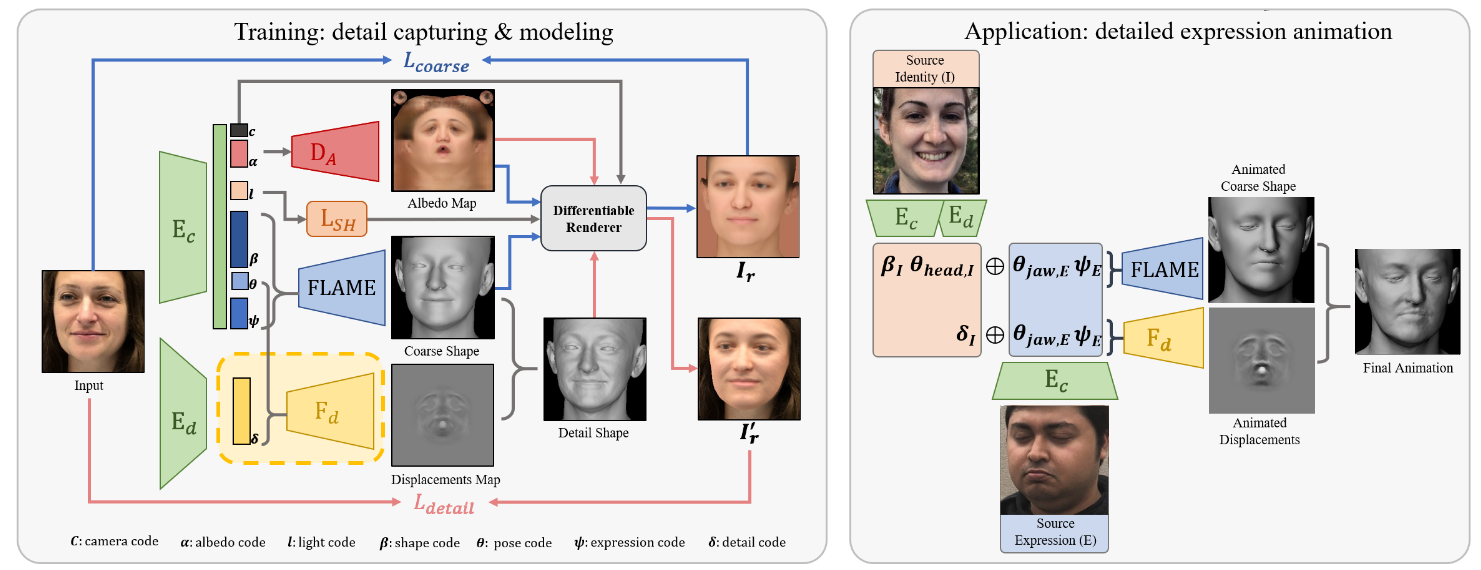
\includegraphics[width=1\linewidth]{deca}
     		 \caption{ DECA tanítás és animáció.
     			    Forrás:\cite{deca}}
                \label{fig:deca}
     	      \end{figure}

            \subsubsection{Kódoló} \label{Kódoló}
    	        Első lépésként egy durva rekonstrukciót a FLAME modelltérben \cite{flame}
                tanítanak be $analysis$-$by$-$synthesis$ módon: egy bemenetként átadott \textit{I} 2D-s képből látens kódot készítenek, ezt dekódolják annak érdekében, hogy egy $I_{r}$ 2D-s képet hozzanak létre, valamint minimalizálják a szintetizált és a bemeneti kép közötti különbséget.
            
    	        Az ábrán \ref{fig:deca} látható módon, egy $E_{c}$ kódolót tanítanak be, amely egy ResNet50 \cite{liwen} hálózatból, és egy azt követő teljesen összekapcsolt rétegből áll, egy alacsony dimenziós látens kód regressziója céljából. Ez a látens kód tartalmazza a $\omega$ (identitás), $\psi$ (arckifejezés), $\theta$ (póz) FLAME \cite{flame} paramétereket (azaz reprezentálja a durva geometriát), az albedó együtthatókat $\alpha$, a kamera $c$ és a megvilágítási $l$ paramétereket.
    
                A durva rekonstrukcióhoz hasonlóan egy $E_{d}$ kódolót is betanítanak (amelynek architektúrája megegyezik a $E_{c}$-vel), hogy a bemeneti képet egy 128 dimenziós látens kódba kódolja, amely a személyre jellemző részleteket reprezentálja. 
    
    
                A kódolás folyamata a következőképpen mükődik:
                \begin{itemize}
    	           \item A bemeneti kép először egy sor konvolúciós rétegen halad át, amelyek magas szintű jellemzőket vonnak ki a képből. Minden egyes konvolúciós réteget egy csoportos normalizáló réteg és egy aktivációs függvény követ a normalizáláshoz és a nemlinearitás bevezetéséhez a konvolúciós réteg kimenetén.
                
    	           \item A konvolúciós rétegek kimenetét ezután kilapítják, és egy teljesen összekapcsolt rétegen vezetik át, ami csökkenti a jellemzővektor dimenzióját.
                
    	           \item A teljesen összekapcsolt réteg kimenete ezután több további teljesen összekapcsolt rétegen halad át, amelyek mindegyikét egy tételes normalizáló réteg és egy aktiváló függvény követi. Ezek a rétegek a jellemzővektort egy alacsonyabb dimenziós látens kódra képezik le a látens térben.
                
    	           \item Az utolsó, teljesen összekapcsolt réteg kimenete a látens kód.
    	           
                \end{itemize}
    
            \subsubsection{Dekódoló} \label{Dekódoló}
    
                A dekódolási folyamat során a bemeneti látens kód először egy sor teljesen összekapcsolt rétegen halad át, hogy egy nagydimenziós jellemzővektort hozzon létre. Ezt a jellemzővektort ezután egy 3D-s tenzor alakjára alakítják át, majd egy sor dekonvolúciós rétegen vezetik át a tenzor felskálázásához és a kimeneti kép előállítása érdekében.
    
                A dekódoló dekonvolúciós rétegei lényegében a kódoló konvolúciós rétegeinek ellentétes műveletét végzik, azaz a bemeneti tenzort nagyobb felbontásra mintavételezik. Az egyes dekonvolúciós rétegek kimenete egy csoportos normalizáló rétegen és egy aktivációs függvényen halad át a nemlinearitás bevezetése és a kimenet normalizálása érdekében.
    
                A dekódoló végső kimenete a kívánt pózt tartalmazó rekonstruált kép. A dekódoló hálózat egy részletes $UV$ elmozdulási térképpel $D$ egészíti ki a durva $FLAME$ geometriát. A látens kódot $\delta$
     	        a $FLAME$ $\psi$ arckifejezés és állkapocs póz $\theta_{jaw}$ paramétereivel kapcsolják
     	          össze, majd $F_{d}$ az imént említett paraméterekből előállítja $D$-t. 
                $F_{d}$ a látens kódot $\delta$ felhasználva szabályozza a statikus személyspecifikus részleteket. Kihasználja a durva rekonstrukcióból kapott arckifejezés $\psi$, és az állkapocs $\theta_{jaw}$ paramétereket a dinamikus, kifejezésektől függő ráncok részleteinek rögzítése érdekében. A rendereléshez $D$-t normáltérképpé alakítják.

            \subsubsection{Részletkonzisztencia veszteség}
    	 
        	    \begin{figure}[h]	
        	 	     \centering
        	 	     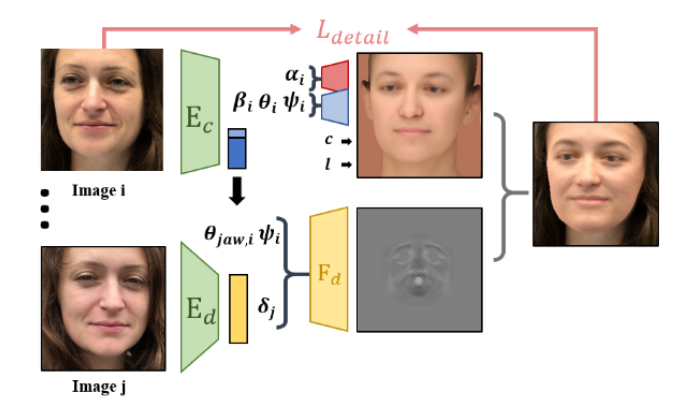
\includegraphics[width=1\linewidth]{ldetail}
        	 	     \caption{Részletkonzisztencia veszteség \\
        	 		    Forrás:\cite{deca}}
                  \label{fig:ldetail}
    	        \end{figure}
    
                Yao Feng és tsai. az identitás-függő és a kifejezésektől függő részletek
     	        szétválasztása érdekében egy új részletkonzisztencia veszteség függvényt
     	        javasolnak. A metódus nélkül a személyspecifikus látens kód $\delta$ rögzíti az
                identitástól és a kifejezésektől függő részleteket. 
                Ebből kifolyólag a rekonstruált részletek nem repozicionálhatóak a FLAME állkapocs póz $\theta_{jaw}$ és arckifejezés $\psi$ paramétereinek megváltoztatásával. Amennyiben adott két kép $I_{i}$ és $I_{j}$ ugyanarról az alanyról ($c_{i} = c_{j}$), a veszteséget a következőképpen határozzuk meg:
        
                \begin{equation*}
                L_{dc} = L_{detail}(I_{i}, R(M (\beta_{i}, \theta_{i}, \psi_{i}), A(\alpha_{i}), F_{d}(\delta_{j} , \psi_{i}, \theta_{jaw,i}), l_{i}, c_{i}))
                \end{equation*}
            
         	      , ahol $\beta_{i},$ $\theta_{i},$ $\theta_{jaw,i},$ $\alpha_{i},$ és 
                $c_{i}$ $I_{i}$ paraméterei, valamint $\delta_{j}$ $I_{j}$ részletkódja.

            \subsubsection{Tanítás}
                Ebben az alfejezetben a(z) \ref{fig:deca}. ábrán szemléltetett $DECA$ modellt vizsgáljuk meg.
     	          A tanítás során (bal oldali doboz) a $DECA$ minden egyes képhez
     	          az arc alakjának rekonstruálásához szükséges paramétereket becsli meg az
     	          alakkonzisztencia információ segítségével (a kék nyilakat követve), majd
     	          a részletkonzisztenica információ (a piros nyilakat követve) kihasználásával
     	          megtanul egy kifejezésfüggő elmozdulási modellt. A sárga doboz tartalmazza
     	          az elmozdulási konzisztencia-veszteséget, amelyet részletesebben
                a(z) \ref{fig:ldetail}. ábra szemléltet.
     	          A tanítás után a $DECA$ animál egy arcot (\ref{fig:deca}. ábra, 
                jobb oldali doboz) a rekonstruált forrásidentitás alakjának, fejpózának, részletkódjának valamint a forráskifejezés állkapocs pózának és arckifejezési paramétereinek kombinálásával annak érdekében, hogy egy animált durva alakot és elmozdulási térképet kapjon. A modell kimenete egy animált
     	          részletes alakzat.

                A betanítási folyamat a következő lépésekből áll:
                    \begin{itemize}
                        \item \textbf{Az adatok előfeldolgozása}: Az adatok előfeldolgozása annak biztosítása érdekében, hogy azok megfelelően igazodjanak és normalizálódjanak, valamint átméretezzék és körülvágják az arcot.
    
                        \item \textbf{Kódolás} Ahogy a fentiekben említettük \ref{Kódoló}, a DECA modell egy kódolót használ a bemeneti arc alacsony dimenziós reprezentációvá alakításához. 
    
                        \item \textbf{Dekódolás} Ahogy a fentiekben említettük \ref{Dekódoló} Az alacsony dimenziós reprezentációt ezután egy dekóderbe tápláljuk, amely rekonstruálja az eredeti arcot egy adott arckifejezéssel
    
                        \item \textbf{Veszteségfüggvény}: A rekonstruált arc és a bemeneti arc közötti különbséget több veszteségfüggvény segítségével számszerűsítjük. Ezek a veszteségfüggvények a neurális hálózat súlyainak beállítására szolgálnak, hogy minimalizálják a rekonstruált arc és a bemeneti arc közötti különbséget.
    
                        \item \textbf{hiba-visszaterjesztés}: A neurális hálózat súlyainak frissítése hiba-visszaterjesztéssel történik, amely a veszteségfüggvény gradiensének kiszámítását jelenti a súlyok tekintetében, valamint a súlyok ennek megfelelő beállítását.
    
                        \item \textbf{Iteratív tanítás}: A tanítási folyamatot több cikluson keresztül addig ismétlik, amíg a modell nem konvergál egy megfelelő teljesítményszintre.
                    \end{itemize}
                
            \subsubsection{Adathalmazok}
                A $DECA$-t három nyilvánosan elérhető adathalmazon tanítják:
     	              \begin{itemize}
     	            	\item VGGFACE2
     	            	\item BUPT-Balancedface
     	            	\item VoxCeleb2
     	              \end{itemize}
    
                A VGGFace2 több, mint 8 ezer alany képeit tartalmazza, átlagosan több,
     	          mint 350 képpel alanyonként. A BUPT-Balancedface 7 ezer képet kínál
     	          etnikumonként, és a VoxCeleb2 pedig 145 ezer videót tartalmaz 6 ezer
     	          különböző alanyról. összességében a DECA-t több, mint 2 millió képpel tanították
     	          be.

            \subsubsection{FLAME modell}

                Mint ahogy korábbiakban megvolt említve a \ref{DECA} fejezetben, a javasolt módszerben a FLAME modellt szintetikus 3D-s arcok generálására használják  az arckifejezések, a póz és a fényviszonyok variációival. Ezeket a szintetikus arcokat ezután a valós világbeli képekkel együtt egy mély neurális hálózat betanítására használják, amely képes megjósolni a FLAME modell paramétereit egy bemeneti kép alapján.

                A FLAME modell egy statisztikai fejmodell \cite{flame}, ami pontosabb és kifejezőbb mint a korábbi fej- és arcmodellek, miközben kompatibilis marad a szabványos grafikus szoftverekkel. A már meglévő modellekkel ellentétben a FLAME explicit módon modellezi a fej tartását és a szemgolyó forgását.

                A FLAME egyesíti a különálló lináris identitásalak és kifejezés tereket $linear$ $blend$ $skinning$-gel (LBS) és a pózfüggő korrektív $blendshape$ alakzatokat, annak érdekében, hogy a nyak, az állkapocs és a szemgolyók mozgathatóak legyenek. Adott arc identitás $\beta \in R^{|\beta|}$, póz $\theta \in R^{3k+3}$ (ahol $k = 4$ a nyak, állkapocs, és szemgolyók ízületeinek száma), és arckifejezés $\psi \in R^{|\psi|}$ paraméterek mellett, a FLAME egy $n = 5023 $ csúcspontot tartalmazó archálót ad kimenetül.

                A modell a következőképpen van definiálva: 

                \begin{equation*}
                    M (\beta, \theta, \psi) = W (T_{p}(\beta, \theta, \psi), J(\beta), \theta, W)
                \end{equation*}

                ahol, a $blendskinning$ függvény $W (T, J, θ, W)$ elforgatja a  $T \in R^{3n}$ csúcsait a $J \in R^{3k}$ ízületek körül, lineárisan finomítva a $W \in R^{k\times n}$ keverési súlyokkal. A $J$ ízületi helyek a $\beta$ identitás függvényeként definiálhatók.

                Továbbá, 
                \begin{equation*}
                    T_{p}(\beta, \theta, \psi) = T + B_{S}(\beta, S) + B_{P}(\theta, P) + B_{E}(\psi, E)
                \end{equation*}

                jelöli a $T$ minta átlagát ”nullpózban” a hozzáadott alak blendshape-ekkel $B_{S} (\beta, S) : R^{|\beta|} \Rightarrow R^{3n}$, pózkorrekciókkal $B_{P}(\theta, P) : R^{3k+3} \Rightarrow R^{3n}$, valamint kifejezés blendshape-ekkel $B_{E}(\psi, E) : R^{|\psi|} \Rightarrow R^{3n}$, a megtanult identitás-, póz- és kifejezésalapokkal (lineáris alterekkel) $S, P$ és $E$. \\

                A legtöbb korábbi módszer figyelmen kívül hagyta a szemeket a
                hozzáigazítás során. Ez torzítja a szemhéjakat és jelentős fotometriai hibákat okoz a szemek régiójában. Következésképpen szemgolyókat adtak hozzá a hálóhoz és bizonyították, hogy ez segíti az igazítási folyamatot.

                Egyik fő szempont, hogy kutatásunkban a FLAME modellt használjuk, az hogy a FLAME betanított modelljeit kutatási célokra nyilvánosan hozzáférhetővé tették, valamint a modell segítségével animálható 3D arcok készíthetőek.

            \subsubsection{Linear Blend Skinning (LBS)}

                A Linear Blend Skinning (LBS) egy népszerű technika a számítógépes grafikában a 3D modellek mozgásának animálására. Az LBS-t egy hálómodell valós idejű deformálására használják, hogy animációkat hozzanak létre, például a karakterek mozgását, arckifejezéseit és ruházatának deformálódását.

                Az LBS alapötlete az, hogy a háló minden egyes csúcspontját egy csontváz csontjaihoz társítja. Minden csonthoz egy transzformációs mátrix tartozik, amely megadja, hogyan mozgatja vagy forgatja az általa befolyásolt csúcsokat. Az animáció lejátszásakor a csontok transzformációit a háló csúcsaira alkalmazzuk, ami a háló deformációját eredményezi, amely követi a csontok mozgását.
                
                Az LBS-ben egy csúcs deformációját az adott csúcsot befolyásoló csontok transzformációinak súlyozott átlaga határozza meg. Az egyes csontok súlyát a csúcsra gyakorolt hatásuk határozza meg, amelyet általában távolság- vagy szögalapú súlyozási függvény segítségével számítanak ki.
                
                A csontok transzformációinak súlyozott átlagát mátrixszorzással számoljuk ki, ami egy új transzformációs mátrixot eredményez, amelyet a csúcsra alkalmazunk. Ez a folyamat a háló minden egyes csúcspontjára megismétlődik, így a teljes háló deformációja követi a csontok mozgását.
                
                Az LBS-t a 3D arcmodell deformálására használjuk az arc tájékozódási pontok vagy a 2D tájékozódási pont detektor által megjósolt tájékozódási pontok mozgása alapján.

                A folyamat a következő lépésekből áll:
                    \begin{enumerate}
                        \item \textbf{Súlyok hozzárendelése minden egyes csúcshoz}: 
                        
                        Ez határozza meg, hogy az egyes csontok milyen mértékben befolyásolják az egyes csúcsokat. 
                    	A súlyok jellemzően olyan értékek halmazaként jelennek meg, amelyek összege minden egyes vertex esetében 1. A DECA-ban ezeket a súlyokat a Softmax nevű módszerrel számítják ki.
                    
                        \item \textbf{Az átalakított csúcspont pozíciójának kiszámítása}: 
                        
                        Az egyes csúcspontok pozícióját az egyes csontok pozíciója és orientációja alapján transzformáljuk. 
                    	Ez úgy történik, hogy a csúcspont pozícióját megszorozzuk az egyes csontokra kiszámított transzformációs mátrixszal. 
                    	A csúcspont végső pozíciója az összes transzformált pozíció összege, az egyes csontokhoz rendelt súlyokkal súlyozva.
                    
                        \item \textbf{A deformáció alkalmazása}: 
                        
                        A transzformált csúcsokat a 3D arcmodell deformálására használjuk. A deformált modellt ezután rendereljük a végső kimenet létrehozásához.
                    \end{enumerate}

                Az LBS egyszerű és hatékony technika a valós idejű animációhoz, és széles körben használják videojátékokban, filmekben és más olyan alkalmazásokban, amelyek dinamikus és interaktív 3D modelleket igényelnek.

                Azonban vannak bizonyos korlátai, például nem képes kezelni az összetett deformációkat. A DECA-ban az LBS-t más technikákkal, például a 
                BlendShape animációval kombinálják, hogy valósághűbb és pontosabb arcanimációkat hozzanak létre.

        \subsection{FOCUS}

            \cite{focus}Chunlu Li és tsai. egy új módszert javasolnak az arc rekonstrukciójára és az elfedések szegmentálására korlátozott vagy tökéletlen képzési adatok felhasználásával, amelyet "gyenge felügyeletnek" nevezünk. A javasolt módszer az arc 3D-s modelljén alapul, és képes pontosan rekonstruálni az arcot még akkor is, ha vannak elfedések, például az arc egyes részeit eltakaró tárgyak.
    
            Az elfedések kezelése érdekében a javasolt módszer egy szegmentálási lépést alkalmaz, amely az arcképet látható és elfedett régiókra osztja. Ezt egy külön neurális hálózat segítségével végzi, amelyet a kép szegmentálására képeztek ki gyenge felügyeleti jelek alapján. Ezek a jelek a szemek, a száj és az orr elhelyezkedéséről szóló előzetes ismereteket, valamint egy sor bináris elfedési maszkot tartalmaznak, amelyek jelzik, hogy az arc mely régiói vannak elfedve.
    
            A javasolt módszert több adathalmazon értékelték, és összehasonlították több más korszerű módszerrel. Az eredmények azt mutatják, hogy a javasolt módszer képes pontosan rekonstruálni az arcot még akkor is, ha vannak elfedések, és felülmúlja a többi módszert a pontosság és az elfedésekkel szembeni robusztusság tekintetében.
    
            Ezenkivül, az általuk használt arc autoencoder lehetővé teszi az arcmodell hatékonyabb illesztését. Ahhoz, hogy növelni tudják a megvilágítással és
     	      más tényezőkkel szembeni robosztusságot, implementáltak egy úgynevezett
     	      perceptuális költségfüggvényt, amellyel a szegmentáló hálózat képes a 
            szemantikus jellemzők helyett csak a független pixeleken keresztül gondolkodni.
    
            Összefoglalva, a javasolt módszer újszerű megközelítést kínál a modellalapú arcrekonstrukció és az okklúziós szegmentáció gyenge felügyelet mellett. A módszer hatékonyan kezeli az okklúziókat, és még akkor is pontos eredményeket produkál, ha korlátozott vagy tökéletlen képzési adatok állnak rendelkezésre.

            \begin{figure}[h]	
     		 \centering
     		 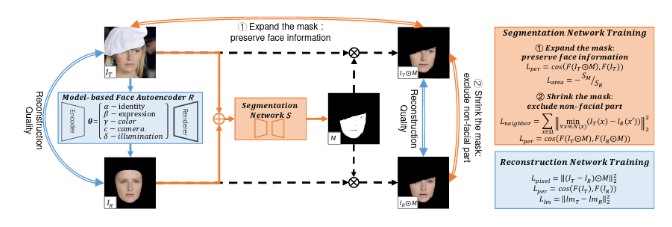
\includegraphics[width=1\linewidth]{focus}
     		 \caption{Chunlu Li et al. által javasolt megközelítés felépítése.
     			    Forrás:\cite{focus}}
                    \label{fig:focus}
     	      \end{figure}

            A fenti ábrán láthatjuk a $FOCUS$ hálózat felépítését.
            Adott egy $I_{T}$ bemeneti kép, a rekonstrukciós hálózat, $R$, megbecsüli a látens
     	      paramétereket és ezt követően egy olyan $I_{R}$ képet állít elő, amely csak az
     	      arcot tartalmazza. Ezután az $I_{T}$ és $I_{R}$ képeket betápláljuk az 
            $S$ szegmentáló hálózatba, amely megjósolja az $M$ szegmentációs maszkot. A szaggatott vonalak azt mutatják, hogy $M$-et arra használják, hogy az $I_{T}$ és $I_{R}$ képekben a becsült kitakaró tényezőket kiszűrjék a képből, ezáltal összerakott kitakarás mentes képeket kapnak, nevezetesen $I_{T}\bigodot M$ és $I_{R}\bigodot M$ .Megfigyelhetjük, hogy Chunlu Li et. al nagy hangsúlyt fektettek bele a robosztus arcrekonstrukcióra kitakarások mellet. A munkánk szempontjából
     	      azért fontos, mert az arcot kitakaró tényezők mindenütt jelen vannak. 
            Ezért is választottuk a $FOCUS$-t, mert nekik sikerült egy speciális modellt implementálni, ami képes kezelni a kitakarásokat anélkül, hogy szükséges lenne nagy mennyiségű adatra vagy olyan erőforrásra, amihez nincs hozzáférésünk.
     	      A továbbiakban részletesebben megvizsgáljuk a $FOCUS$ építőelemeit és
     	      együttműködésüket.

            Ahogy, már korábban is említve volt, a $FOCUS$ célja 3D-s
     	      arcrekonstrukció egyetlen képből, súlyos kitakarások esetén is. Ezen kihívást
     	      jelentő probléma megoldásához egy modellalapú arc autokódolót, $R$-t, és
     	      egy szegmentáló hálózatot, $S$-t implementáltak, ahogyan az a fenti ábrán is
     	      szemléltetve van.
    
            Az arc rekonstrukciójához a szegmentációs maszk a modellillesztés során
     	      kivágja a becsült kitakarásokat, így a rekonstrukciós hálózatot robosztussá
     	      teszi a kitakarásokkal szemben. A szegmentáláshoz a rekonstruált eredmény
     	      referenciaként szolgál, növelve a szegmentálás pontosságát.
    
            Ebben a szakaszban megvizsgáljuk hogyan működik a két hálózat,
     	      hogyan kapcsolódnak egymáshoz és milyen előnyöket nyújtanak
     	      egymás számára.

            \subsubsection{Modellalapú autoencoder}
        
                \cite{focus}A modellalapú arc autokódoló, $R$, várhatóan rekonstruálja a teljes arc
     	          megjelenését a látható arctartományokból a képen, $I_{T}$-n. 
                Ez egy kódolóból, grafikus renderelőből, és egy dekódolóból áll. A kódoló megbecsüli a látens parmétereket $\theta = [\alpha, \gamma, \phi, c] \in R^{257}$, azaz a 3D alak $\alpha \in R^{144}$, a 3DMM textúrája 
                $\gamma ∈ R^{80}$, a megvilágítás $\phi ∈ R^{27}$, és a jelenet kamera paraméterei $c ∈ R^{6}$. Adott látens parméterekkel a dekódoló a bemeneti képen látható arcképét állítja elő $I_{R} = R(\Theta)$. Majd ehhez egy olyan felügyelet nélküli szegmentáló hálózatot vezetnek be, melynek kimenetelét a modellillesztés során a kitakarások elfedésére lehet használni, és így az autokódolót robosztussá teszi a kitakarásokkal szemben.

            \subsubsection{Szegmentációs hálózat}
    
                \cite{focus}A szegmentáló hálózat, $S$, veszi az $I_{T}$ képet és a szintetizált képet, $I_{R}$-t, bemenetként, és megjósolja a bináris maszkot, $M = S(I_{T} , I_{R}$, annak leírására, hogy egy pixel az arcot ábrázolja-e $(1)$ vagy nem $(0)$. Mivel az $I_R$ tartalmazza a becsült arcot, előzetes tudást biztosít a szegmentáló hálózatnak és segíti a becslést.
     	
     	          Az arc autokódoló és a szegmentáló hálózat a tanítás során össze 
                vannak kapcsolva olyan módon, hogy egy szinergikus hatást váltanak ki, ami a szegmentálást pontosabbá teszi és a rekonstrukciót robosztussabbá teszi kitakarások jelenlétében.

            \subsubsection{U-Net}
    
                A munkánkban a szegmentáló nagy szerepet játszik, ezért is szeretnénk jobban belemenni a a szegmentáló hálózat részleteibe.
    
                Ebben a szekcióban \cite{unet}Ronneberger és tsai. munkája alapján bemutatjuk az U-Net architektúrát, amelyet a saját megvalósításunkban a szegmentációs maszk elkészítésére, optimalizálására használunk fel. 
    
                A konvolúciós hálózatok tipikus felhasználási területe az osztályozási feladatok, ahol a kép kimenete egyetlen osztálycímke. Azonban számos vizuális feladatban, különösen az orvosbiológiai képfeldolgozásban, a kívánt kimeneti eredménynek tartalmaznia kell lokalizációt, azaz minden egyes képponthoz osztálycímkét kell rendelni. Továbbá, több ezer tanító kép általában elérhetetlen az orvosbiológiai feladatokban. Ezért Ciresan et al. \cite{ciresan} egy csúszóablakos elrendezést alkalmaztak, hogy prediktálják
                az egyes képpontok osztálycímkéjét az adott képpont körüli lokális régió bemenetként történő megadásával.
    
                Ezt az architektúrát úgy módosították és bővítették, hogy
                nagyon kevés tanítási képpel működjön, és pontosabb szegmentációkat eredményezzen.
                Az alapötlet a szokásos szűkülő konvolúciós hálózat kiegészítése egymást követő rétegekkel, ahol a pooling operátorokat upsampling operátorok helyettesítik. Ezért ezek a rétegek növelik a kimenet felbontását. A lokalizáció érdekében a magas felbontású jellemzőket kombinálják a szűkülő útvonalról származó felskálázott kimenettel. Egy ezt követő konvolúciós réteg ezután megtanulhatja a kimenet precízebb összeállítását ezen információk alapján. A felfelé mintavételezés rész nagyszámú funkciócsatornával is rendelkezik, ami lehetővé teszi a hálózat számára, hogy a kontextusinformációkat továbbítsa a magasabb felbontású rétegek felé. Ennek következtében, az expanziós útvonal többé-kevésbé szimmetrikus az összehúzódási útvonalhoz képest, és \textbf{U} alakú architektúrát eredményez.
    
                Az UNet egy mélytanulási architektúra, amelyet általában képszegmentálási feladatokhoz használnak. Először 2015-ben mutatta be \cite{unet}Olaf Ronneberger, Philipp Fischer és Thomas Brox az "U-Net: Convolutional Networks for Biomedical Image Segmentation" című tanulmányukban.
    
                Az UNet architektúra egy kódoló és egy dekódoló hálózatból áll. A kódoló hálózat egy sor konvolúciós és összevonó rétegből áll, amelyek lemintavételezik a bemeneti képet, és kivonják belőle a jellemzőket. A dekódoló hálózat felfelé konvolúciós és összekapcsoló rétegek sorozata, amelyek a kép eredeti felbontására felmintavételezik a jellemzőket, és szegmentálási maszkot generálnak.
    
                Az UNet architektúrát úgy tervezték, hogy kezelni tudja az osztályok kiegyensúlyozatlanságának problémáját a képszegmentálási feladatokban, ahol az egyes osztályokba tartozó pixelek száma jelentősen változhat. E probléma megoldására az UNet architektúra a kódoló és a dekódoló hálózatok közötti kihagyásos kapcsolatokat használja, amelyek lehetővé teszik a dekódoló számára, hogy a szegmentációs maszk finomításához a kódolótól származó nagy felbontású jellemzőket használja. Az UNet architektúra emellett "vágási" technikát alkalmaz a konvolúciós és összevonó rétegek használatakor fellépő határhatások csökkentésére.
    
                Az UNet architektúrát széles körben használják különböző orvosi képalkotó alkalmazásokban, mint például a tumorok felismerése, az agy szegmentálása és a sejtek szegmentálása. Más területeken is  alkalmazták, például a természetes jelenetek szegmentálásában, ahol ígéretes eredményeket mutatott.
    
                A hálózat felépítését a(z) \ref{fig:unet}. ábra szemlélteti. A rendszer egy szűkülő (bal oldal) és egy bővülő útvonalból (jobb oldal) áll. Az összehúzódó útvonal a konvolúciós hálózatok tipikus architektúráját követi.  Ez a következő lépések ismételt meghívásából áll: 
                két 3x3-as konvolúció, melyeket egy-egy ReLU és egy 2x2 max pooling művelet követ. Minden lefelé mintavételezést a jellemzőcsatornák duplázása következik. 
    
                Az expanzív útvonal minden lépése a jellemzőtérkép felmintavételezéséből áll, amelyet egy 2x2-es konvolúció követ, amely megfelezi a jellemzőcsatornák számát, majd egy konkatenáció a megfelelően levágott jellemzőtérképpel a kontraháló útvonalról, és két 3x3-as konvolúció, amelyet egy-egy ReLU követ. A vágásra a határpixelek elvesztése miatt van szükség minden egyes konvolúcióban. Az utolsó rétegben egy 1x1-es konvolúciót használnak minden egyes 64 komponensű jellemzővektor a kívánt számú osztályhoz való kötéséhez. Összességében a hálózat 23 konvolúciós rétegből áll.
    
                Összességében az UNet egy nagy teljesítményű mélytanulási architektúra, amelyet gyakran használnak képszegmentálási feladatokra, különösen az orvosi képalkotás területén. 
        
                \begin{figure}[h]	
     	              \centering
     	        	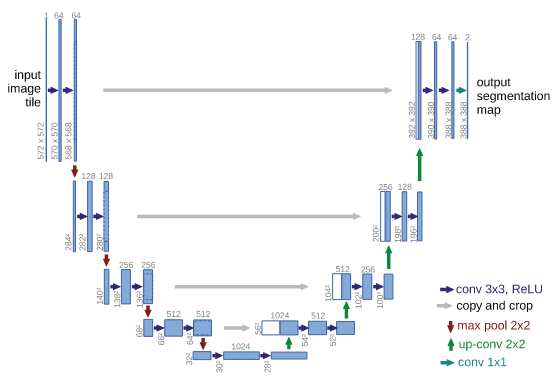
\includegraphics[width=1\linewidth]{unet}
     	        	\caption{U-Net felépítése
     	        		Forrás:\cite{unet}}
                    \label{fig:unet}
     	        \end{figure}
 	
            \subsubsection{Tanítás}
            
         	      Az arc autokódoló és a szegmentáló hálózat kölcsönös függőségei miatt 
                egy $Expectation − Maximization(EM)$ típusú stratégiát alkalmaztak,
         	      ahol a két hálózatot váltakozva tanították be. Ez lehetővé tette a stabil
         	      konvergenciát a betanítási folyamat során. Mint más EM típusú tanítási
         	      stratégiákhoz hasonlóan, a tanítási folyamatuk a modell paraméterinek
         	      durva inicializálásával kezdődik, amely felügyelet nélküli módon történik.
         	
         	      A szegmentáló hálózat tanításakor az arc autokódoló paraméterei
         	      rögzítettek és csak a szegmentáló hálózatot optimalizálják. Alapvetően 
                négy költségfüggvényt javasolnak, amelyek kikényszerítik a képek közötti hansolóságokat. A költségfüggvények dolga hogy, eldöntse egy adott pixelről hogy az arc része vagy sem. Ezek perceptuális szinten vagy pixel szinten dolgoznak, hogy teljes mértékben kihasználják a vizuális nyomokat.
         	
         	      Betanítás során a szegmentáló hálózat feladata, hogy egyensúlyt
         	      keressen az olyan képpontok elvetése között, amelyeket az autokódoló nem
         	      tud jól értelmezni és az olyan képpontok megőrzése között, amelyek fontosak
         	      a bemeneti kép és az előállított arc perceptuális reprezentációjának 
                megőrzése érdekében. Ezáltal nincsen szükség a kitakarások felügyeletére.
         	
         	      Az autkódoló betanítása során, tovább optimalizálták a kódoló paramétereit, 
                közben a szegmentáló hálózat rögzítve van. Az autokódolóhoz az alábbi költségfüggvények tartoznak:
        
                \begin{equation*}
                    L_{pixel} = \parallel (I_{T} − I_{R}) \bigodot M \parallel _{2}^{2} 
                \end{equation*}
                
                \begin{equation*}
                    L_{per} = \cos(F(I_{T}), F(I_{R}))    
                \end{equation*}
                
                \begin{equation*}
                    L_{lm} = \parallel lm_{T} - lm_{R} \parallel _{2}^{2}  
                \end{equation*}
            \subsubsection{Adathalmazok}
            
             	Az általuk felhasznált adatbázisok a CelebA-HQ és az AR adathalmaz.
             	Ezek segítségével értékelik az illesztés és az arcszegmentlás hatékonyságát.
             	Az alakrekonstrukció kiértékelésére a NoW adatbázis
             	részhalmazait használták.
     	
             	\begin{figure}[h!]	
             		\centering
             		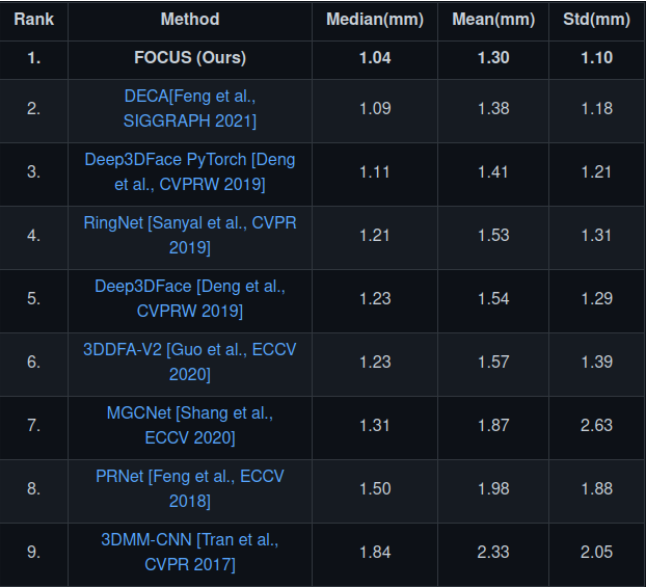
\includegraphics[width=1\linewidth]{now}
             		\label{fig:now}
             		\caption{NoW Challenge benchmark eredményei
             			Forrás: https://github.com/unibas-gravis/Occlusion-Robust-MoFA}
             	\end{figure} 
              
        \subsection{Renderelés}

            A renderelés mind az \cite{focus}Occlusion-Robust MoFA, mind a \cite{deca}DECA projektben fontos, mivel lehetővé teszi a neurális hálózati modellek tanításához szükséges valósághű szintetikus képek létrehozását, valamint a 3D-s tárgyak vagy animált arcok valósághű vizuális reprezentációjának előállítását. A renderelés minősége mindkét projektben jelentős hatással van a végső kimenet pontosságára és valósághűségére.

            Mi ebben a fejezetben inkább \cite{deca}Yao Feng és tsai. által ajánlott módszert akarjuk jobban megvizsgálni, mivel a mi munkánk arcrekonstrukciós hálózata az ő munkájukon alapszik.

            A DECA projekt szempontjából a renderelés azért fontos, mert ez az utolsó lépés az arc rekonstrukciós folyamatában, amely az animált arc valósághű 2D-s képét állítja elő.

            A rendszer az arc időbeli mozgását és deformációját egy mély neurális hálózati modell segítségével rögzíti, amely a bemeneti képek vagy videoképek alapján megjósolja egy 3D-s arcmodell paramétereit. Maga a 3D arcmodell azonban nem közvetlenül megfigyelhető, ezért 2D képpé kell renderelni, hogy az arcanimáció vizuális megjelenítése létrejöjjön.
            
            A renderelés minősége jelentős hatással van a végeredmény realizmusára és hihetőségére. Egy kiváló minőségű renderelőmotor képes valósághű fény- és árnyékhatásokat, pontos bőrszínt és sima mozgást produkálni, amelyek mind hozzájárulnak az animált arc általános vizuális hűségéhez.
            
            A DECA-ban használt differenciálható renderelő továbbá lehetővé teszi a renderelt képek vagy videóképek gradiensének kiszámítását a bemeneti 3D geometria és más renderelési paraméterek tekintetében, lehetővé téve az arc teljesítményének rögzítéséhez használt neurális hálózati modellek végponttól végpontig tartó tanítását.

            \subsubsection{Differenciálható renderelő}

                A differenciálható renderelő a DECA projekt kulcsfontosságú eleme, és a korábban említettek alapján, láthajuk hogy kulcsfontosságú szerepe van.

                 Ebben a fejezetben Kato és tsai. \cite{diffrenderer} kutatása alapján bemutatjuk a differenciálható renderelő alapelvét.

                A legtöbb 3D becslési módszer a felügyelt tanítási rendszerekre és költséges címkézésekre támaszkodnak, ami
                a 3D megfigyelések összes paraméterének összegyűjtését jelentősen megnehezíti. A megközelítések egyike a grafikus renderelési folyamatok integrálása a neurális hálózattal működő rendszerekbe. Ez lehetővé teszi az átalakítást és a 3D becslések beépítését a 2D képi szintű információkba.

                A differenciálható renderelés (DR) olyan technikák családját alkotja, amelyek a renderelési folyamat hasznos gradienseinek kinyerésével végponttól-végpontig tartó optimalizálás céljából integrációt valósítanak meg. A renderelés differenciálásával a DR áthidalja a szakadékot
                a 2D és a 3D feldolgozási módszerek között; Lehetővé téve a neurális hálózatok számára, hogy 2D-s vetületeken dolgozva optimalizálják a 3D-s entitásokat. Amint a(z) \ref{fig:diffrenderer}. ábrán látható, a 3D jelenet paramétereinek optimalizálása a gradiensek visszaterjedésével érhető el a renderelési kimenethez képest. 

                Az általános 3D önfelügyeleti modell a renderelő réteg integrálásával a megjósolt jelenetparaméterekhez és a veszteség alkalmazásával a renderelt és a bemeneti kép különböző módokon történő összehasonlításával történik.

                \begin{figure}[h!]	
            		\centering
            		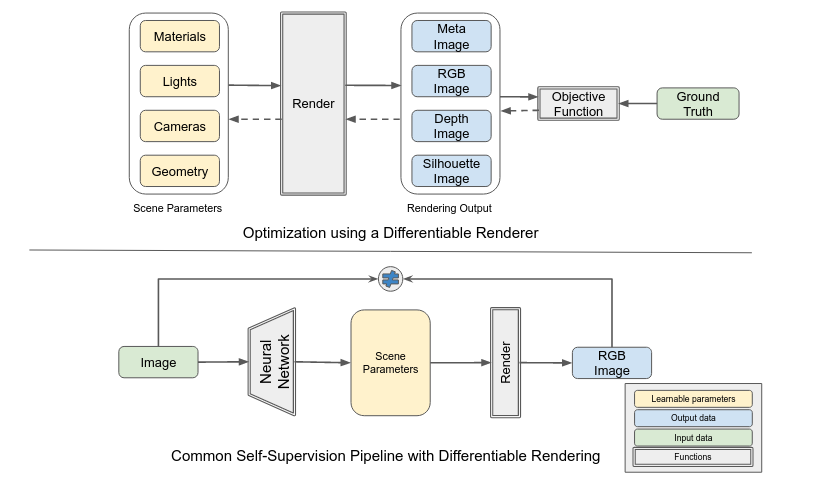
\includegraphics[width=1\linewidth]{diffrenderer}
            		\caption{Általános önfelügyeleti modell differenciálható rendereléssel.\\
                            Forrás: \cite{diffrenderer}}
                    \label{fig:diffrenderer}
            	\end{figure}

                A DECA-ban a differenciálható renderelőt a renderelt arcképek vagy videóképek gradiensének kiszámítására használják a 3D arcgeometria és más modellparaméterek tekintetében. Ez lehetővé teszi a hiba-visszaterjesztést más gradiens-alapú optimalizálási technikák használatát az arc teljesítményének teljes körű rögzítésére szolgáló neurális hálózati modellek betanításához.

                A tanítás során a differenciálható renderelőt szintetikus arcképek vagy videóképek egy sorának renderelésére használják a 3D arcmodellek és a megfelelő kifejezések véletlenszerűen generált készletének felhasználásával. A renderelt képeket vagy videoképeket ezután egy veszteségfüggvény segítségével összehasonlítjuk egy alapigazságkép- vagy videoképkészlettel. A veszteségfüggvény gradienseit a 3D arcmodellek és más modellparaméterek tekintetében a differenciálható renderelő segítségével számítják ki és a modellsúlyok frissítésére használják.
                
                A differenciálható renderelő ilyen módon történő használatával a DECA képes olyan neurális hálózati modelleket tanítani, amelyek képesek megragadni az arckifejezések és a mögöttes 3D arcgeometria közötti összetett kapcsolatot és kiváló minőségű arcanimációkat készíteni a bemeneti képekből vagy videóképekből.

            \subsubsection{Raszterizáló}

                A DECA projekt keretében a raszterizáló a renderelési folyamat utolsó lépésében játszik szerepet, amely a 3D arcmodell 2D képpé vagy videoképpé alakítása. Konkrétan a raszterizáló felelős a 3D arcmodell 2D-s képsíkra történő vetítéséért.

                A raszterizáló a grafikus folyamat egyik összetevője, amelyet a számítógépes grafikában és a játékfejlesztésben gyakran használnak. Úgy működik, hogy az archáló csúcsainak 3D-s koordinátáit egy 2D-s képsíkra vetíti. A vetítés során a 3D koordinátákat 2D képernyőkoordinátákká alakítják át figyelembe véve a kamera perspektíváját és minden egyéb releváns paramétert, például a látómezőt és a képarányt.
                
                Miután az arc hálójának csúcsait kivetítették a 2D-s képsíkra, a raszterizáló a hálót alkotó háromszögeket kitölti a megfelelő színekkel vagy textúrainformációkkal a renderelési folyamat során korábban elvégzett megvilágítási és árnyékolási számítások alapján.
                
                A raszterizáló kimenete egy pixelalapú kép vagy videókép, amely a renderelt 3D arcanimáció részleteit rögzíti.

            \subsubsection{Renderelési folyamat}

                A renderelési folyamat több lépésre bontható:

                \begin{enumerate}
                    \item \textbf{Az arc tájékozódási pontjainak felismerése}: A rendszer először az arc tájékozódási pontjait észleli a bemeneti képeken vagy videóképeken. 

                    \item \textbf{Kép normalizálás}: A bemeneti képeket vagy videoképeket szabványos méretre és felbontásra normalizálják.

                    \item \textbf{3D arc rekonstrukció}: A DECA az észlelt arctájékozódási pontjainak felhasználásával rekonstruálja az arc 3D-s modelljét. A 3D modell csúcspontokból álló hálóból áll, amelyek a 3D térben úgy helyezkednek el, hogy megfeleljenek az arc alakjának és kontúrjainak.

                    \item \textbf{Textúra leképezés}: A 3D arc rekonstrukció után a rendszer textúratérképet alkalmaz a 3D arcmodellre, hogy valósághű bőrszínt és részleteket adjon hozzá.

                    \item \textbf{Világítás és árnyékolás}: A 3D arcmmodellre világítást és árnyékolást alkalmaznak, hogy valósághű fénypontokat és árnyékokat hozzon létre. 

                    \item \textbf{Renderelés}: Végül a DECA rendereli a 3D arcmodellt az alkalmazott textúrával, világítással és árnyékolással, hogy az animált arcról valósághű 2D képet készítsen.
                    
                \end{enumerate}
                
 	      \subsection{Értékelés}

            Mint láthatjuk a fent említett megközelítések mind kiváló eredményeket nyújtanak, de megfigyelhetjük hogy a két munkának a szerzői teljesen különböző motivációval rendelkeztek.
            
         	A $DECA$ főbb motivációja az emberi arc részleteinek megőrzése valamint az arc realisztikus animálhatósága. A $FOCUS$ célja pedig egy gyors modell kialakítása volt, amely korábbi munkákhoz képest jobban kezeli a kitakarásokat. A mi célunk, egy olyan animálható modell kialakítása, amely képes megőrízni a részleteket. Emellett képes konzisztens mükődést nyújtani súlyos kitakarások jelenlétében is.
 	
 	          Tehát a tervezett modell, amit a későbbiekben részletesebben
 	          megvizsgálunk kettő egymást támogató hálózatból áll. Egyik fő 
            épitőeleme a$DECA$ alapján készített rekonstrukciós hálózat. A másik,a $FOCUS$ megközelítésében implementált szegmentációs hálózat. E két hálózaton egy EM típusú stratégiát alkalmazunk a tanítási folyamat során.

            
    \section{Megvalósítás}
 	
 	    

        

 \end{document}